\documentclass[12pt,a4paper]{report}
\usepackage[utf8]{inputenc}
\usepackage{url}

\usepackage{a4wide}
\usepackage{longtable}           % lange Tabellen
\usepackage{graphicx}
\usepackage{amsmath}
\usepackage{multirow}

\usepackage{fancyhdr}

%\bibliographystyle{alpha} % does not work as expected

\pagestyle{fancy}
%\fancyhf{}                              % bisherige Kopf- und Fusszeilen loeschen
\fancyhead[R]{Nico Schottelius}            % rechter Kopfzeileneintrag
%\fancyhead[L]{Projekdokumentation}      % linker Kopfzeileneintrag
%\fancyhead[L]{\thepage}      % linker Kopfzeileneintrag
%\fancyfoot[C]{\thepage}                % Fusszeileneintrag (Seitenzahl zentriert)
\renewcommand{\headrulewidth}{0.4pt}  % Strichstaerke unter der Kopfzeile
% ----------------------------------------------------------------------------
% let's start
\begin{document}
\title{Development of a secure, peer-to-peer, decentralised anonymous chat system}
\date{\today}
\author{Nico Schottelius (nico-zhaw.ch (o) schottelius.org)}
% ----------------------------------------------------------------------------
\maketitle
\newpage
% ----------------------------------------------------------------------------
% Inhaltsverzeichnis
\tableofcontents
\listoftables
\listoffigures
\newpage

% ----------------------------------------------------------------------------
% ----------------------------------------------------------------------------
\chapter{Introduction}

Anonymous communication networks were first intro-
duced by David Chaum in his seminal paper [10] describing
the mix as a fundamental building block for anonymity.
(aus tor2)

\subsection{Abstract}
hier oder weiter oben? - siehe lisa vortrag!

\subsection{Abbreviations}
\subsection{Starting Position}
local, skype, untrustworthy

\subsection{Motivation}
From EBS + EOF

\subsection{Objectives}
From EOF + Latency "`low"', eventual consistency
\subsubsection{Steganographic}
Not for hiding, but to support longer überleben?
http is pretty well suited for this.
mixing with smtp, imap, pop3, tcp. etc.



% ----------------------------------------------------------------------------
\chapter{Analysis and Comparision of Chat Systems}

    1. Detailed analysis and comparison of open and legacy chat systems
        to summarise current chat system features and their
        security characteristics.


% ----------------------------------------------------------------------------
\section{IRC}
\subsection{History}

Since 1989 deleoped\ref{rfc2810},
first formally documented in May 1993 by RFC 1459\ref{rfc1459}.

\begin{quote}
All client-to-server IRC protocols in use today are descended from the protocol implemented in the irc2.4.0 version of the IRC2 server, and documented in RFC 1459. Since RFC 1459 was published, the new features in the irc2.10 implementation led to the publication of several revised protocol documents (RFC 2810, RFC 2811, RFC 2812 and RFC 2813); however, these protocol changes have not been widely adopted among other implementations.\ref{irc-wp}
\end{quote}

% ----------------------------------------------------------------------------
\subsection{Architecture}
central server, server network
IRC, the \textit{Internet Relay Chat}, has been developed since 1989
and is defined in severals Internet RFCs.\footnote{See \cite{rfc1459}, 
\cite{rfc2810}, \cite{rfc2812} and \cite{rfc2813}.}
IRC networks consist of IRC servers and IRC clients:

\begin{verbatim}
                       1--\
                           A        D---4
                       2--/ \      /
                             B----C
                            /      \
                           3        E

   Servers: A, B, C, D, E         Clients: 1, 2, 3, 4

                    [ Fig. 1. Sample small IRC network ]

\end{verbatim}\footnote{Source: \cite{rfc2810}}
IRC is organised centrally, as stated in \cite{rfc2810}:
\begin{quote}
The IRC protocol provides no mean for two clients to directly
communicate.  All communication between clients is relayed by the
server(s).
\end{quote}

There is, however, an unstandartised client extension named 
\textit{Direct Client-to-Client} (DCC) available in most IRC clients
that enables direct connections.\footnote{See \cite{dcc}, \cite{dcc2}.}

% ----------------------------------------------------------------------------
\subsection{Security}
SSL is being used in some networks, but not standartised. [nico]
optional encryption.
% ----------------------------------------------------------------------------
\section{Silc}
SILC Project develops the Secure Internet Live Conferencing protocol (SILC),
\url{http://silcnet.org/general/}
\url{http://silcnet.org/support/documentation/specs/}

central
\url{http://silcnet.org/support/documentation/wp/silc_protocol.php}


% ----------------------------------------------------------------------------
\section{Skype}
More VoIP
% ----------------------------------------------------------------------------
\section{MSN}
More VoIP
% ----------------------------------------------------------------------------
\section{ICQ}
More VoIP


% ----------------------------------------------------------------------------
\section{Security features and Comparision}

\begin{longtable}{|c|c|c|}
\caption{Chat system comparision with security features}\\
\hline
\textbf{Name} & \textbf{IRC} & \textbf{SILC}\\
\hline
\textbf{Single point of attack} & yes & yes\\
\hline
\textbf{Encrypted traffic} & optional & yes\\
\hline
\end{longtable}

All the solutions with objectives.

\chapter{Analysis of related communication protocols}

% ----------------------------------------------------------------------------
\section{Mix networks}
Mix networks are also known as onion routing or digital mixes and
were invented by David Chaum in 1981.\cite{Chaum:1981:UEM:358549.358563}
\begin{figure}
    \centering
    \caption[Mixes: Packet Flow]{Mixes: Packet Flow\\Image source \url{http://upload.wikimedia.org/wikipedia/en/2/23/Decryption_mix_net.png}}
    \label{mixesflow}
    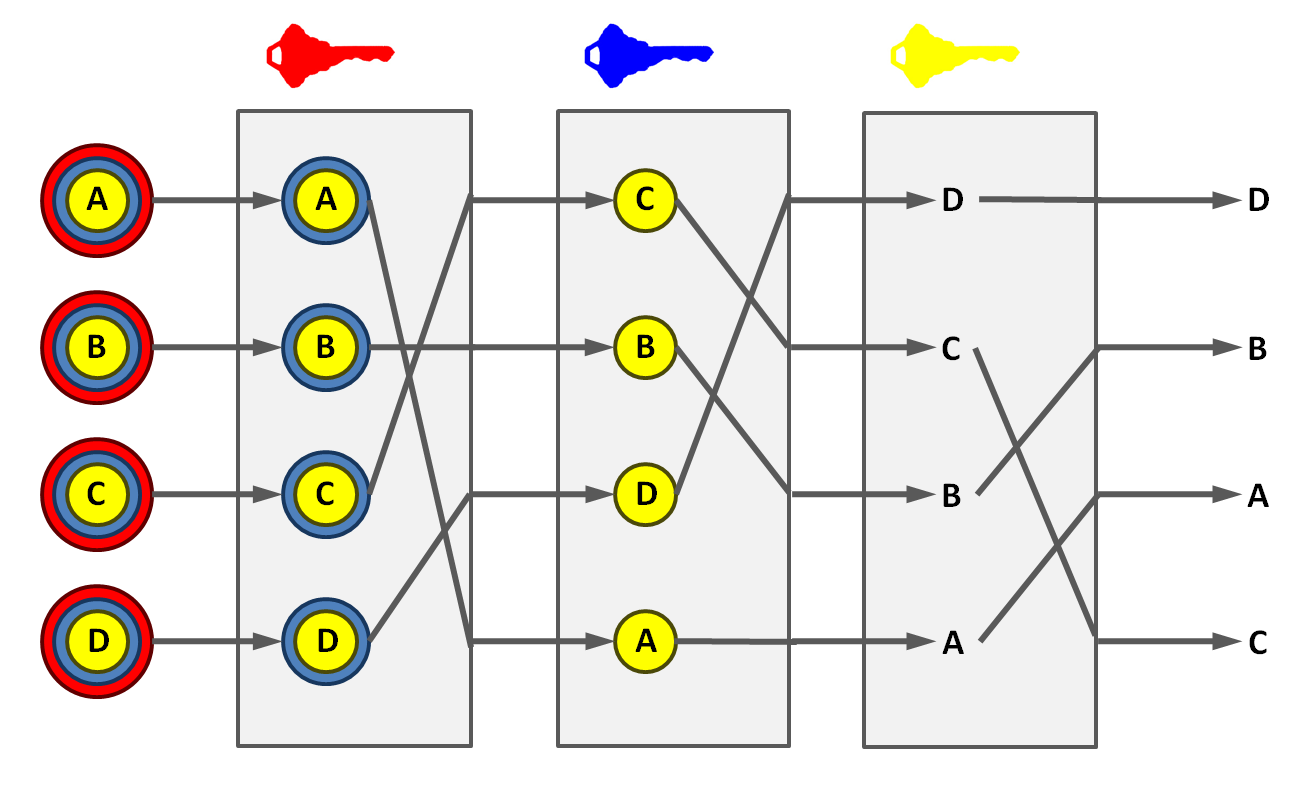
\includegraphics[scale=0.3]{Decryption_mix_net.png}
\end{figure}
The base of Mixes is the multiple encrypted packet that is send through a
number of peers (the mixes) as shown in figure \ref{mixesflow}.
Every peer decrypts the message, which reveals which is the next peer
to send the packet to. Using this method, every peer only knows about
its predecessor and successor. For encryption Public-Key-Cryptography (RSA) is used.
The original approach was focussing on Mixes for e-mail delivery.
% Patent \url{http://patft1.uspto.gov/netacgi/nph-Parser?Sect1=PTO2&Sect2=HITOFF&p=1&u=%2Fnetahtml%2FPTO%2Fsearch-bool.html&r=1&f=G&l=50&co1=AND&d=PTXT&s1=6266704.PN.&OS=PN/6266704&RS=PN/6266704}
% ----------------------------------------------------------------------------
\section{Tor}
The Tor network has been published in 2004
at the 13th USENIX Security Symposium by Roger Dingledine, 
Nick Mathewson and Paul Syverson.\cite{tor}
The idea behind Tor is to provide a general purpose, 
low latency anonymising network stack.
They explicitly do not include application level anonymity
(like stripping user agent information from a http request) and
reason this to leave it up specialised projects.
Tor does (by design) offer no protection against end-to-end attacks
(for instance using traffic analysis) to support low latency applications.
The Tor software provides access to its network via
a SOCKS proxy interface.
Tor does not use the traditional mix approach:
\begin{quote}
Rather than using a single multiply encrypted
data structure (an onion) to lay each circuit, Tor now uses an
incremental or telescoping path-building design, where the
initiator negotiates session keys with each successive hop in
the circuit.\footnote{Quote from \cite{tor}.}
\end{quote}
%\url{http://en.wikipedia.org/wiki/Onion_routing}
% Reply onions have been replaced by a rendezvous system, 
%Generic transport protocol.
%    Separation of “protocol cleaning” from anonymity:

%Onion Routing originally required a separate “application
%proxy” for each supported application protocol—most of
%which were never written, so many applications were never
%supported.
%Tor uses the standard and near-ubiquitous
%SOCKS proxy interface, allowing us to support most
%TCP-based programs without modification. Tor now relies on
%the filtering features of privacy-enhancing application-level
%proxies such as Privoxy [39], without trying to duplicate those
%features itself.
%% No mixing, padding, or traffic shaping (yet): Onion
%% Routing originally called for batching and reordering cells
%% as they arrived, assumed padding between ORs, and in later
%% designs added padding between onion proxie
%% 
%% 
%% Perfect forward secrecy: In the original Onion Routing
%% design, a single hostile node could record traffic and later
%% 
%% ...
%% 
%% 
%% Not secure against end-to-end attacks: Tor does not
%% claim to completely solve end-to-end timing or intersection
%% attacks. Some approaches, such as having users run their own
%% onion routers, may help; see Section 9 for more discussion.
%% 
%% \cite{tor}
% ----------------------------------------------------------------------------
\section{Off-the-Record Messaging (OTR)}
Off-the-Record Messaging (OTR) has been introduced by
Nikita Borisov, Ian Goldberg and Eric Brewer in 2004.\cite{otr}
In contrast to other approaches OTR does not rely on long term
keys as usually used in Public-Key-Cryptography. OTR instead
uses short time keys, to prevent decryption of sniffed messages,
if access to the private key is gained after some time.

Furthermore OTR includes measures to include repudiability, though
provide authentication during a session using
message authentication codes (MAC).
OTR works as a drop in for existing chat programs and offers auto-detection
if the other side is capable of using OTR as well.
%As of OTR 3.1 the protocol supports mutual authentication of users using a shared secret through the socialist millionaire protocol. This feature makes it possible for users to verify the identity of the remote party and avoid a man in the middle attack without the inconvenience of manually comparing public key fingerprints through an outside channel. 
% \url{http://de.wikipedia.org/wiki/Off-the-Record_Messaging}
% ----------------------------------------------------------------------------
\section{Freenet}
Freenet has been published in 2001 by
Ian Clarke , Oskar Sandberg , Brandon Wiley and Theodore W. Hong.\cite{freenet}
Its primary use the anonymous storage (and retrieval) of files.
Freenet is described as follwing:
\begin{quote}
Freenet is free software which lets you anonymously share files, browse and publish "freesites" (web sites accessible only through Freenet) and chat on forums, without fear of censorship. Freenet is decentralised to make it less vulnerable to attack, and if used in "darknet" mode, where users only connect to their friends, is very difficult to detect.\footnote{Quote from \url{https://freenetproject.org/whatis.html}}
\end{quote}
% ----------------------------------------------------------------------------
\section{I2P}
The I2P project, originally Invisible Internet Project, is supposed to be
"`a scalable framework for anonymous communication"'.\cite{i2p} 
It is described on the website as following:
\begin{quote}
I2P initially began in Feb 2003 as a proposed modification to Freenet to allow it to use alternate transports, such as JMS, then grew into its own as an 'anonCommFramework' in April 2003, turning into I2P in July, with code being written in earnest starting in August '03. I2P is currently under development, 
following the roadmap.\footnote{Quote from \url{http://www.i2p2.de/how_intro}.}
\\
...
\\
I2P is a scalable, self organizing, resilient packet switched anonymous network layer, upon which any number of different anonymity or security conscious applications can operate. Each of these applications may make their own anonymity, latency, and throughput tradeoffs without worrying about the proper implementation of a free route mixnet, allowing them to blend their activity with the larger anonymity set of users already running on top of I2P.\footnote{Quote from \url{http://www.i2p2.de/techintro.html}.}
\end{quote}
Although the overall of the impression of the website indicates that it may provide a
reasonable base for anonymous communications, the lack of a central architecture or
design paper makes it hard to judge about it.
%% I2P (initially short for Invisible Internet Project)
%% 
%% I2P is an anonymizing network, offering a simple layer that identity-sensitive applications can use to securely communicate. All data is wrapped with several layers of encryption, and the network is both distributed and dynamic, with no trusted parties.
%% 
%% Many applications are available that interface with I2P, including mail, peer-peer, IRC chat, and others.
%% 
%% 
%%  a low latency, fully distributed, autonomous, scalable, anonymous, resilient, and secure network
%% 
%%   I2P is a low latency mix network, 
%% 
%% 
%% \url{http://en.wikipedia.org/wiki/I2P}
%% 
%% \url{http://www.i2p2.de/_static/images/endToEndEncryption.png}
%% 
%% The first time a client wants to contact another client, they make a query against the fully distributed "network database" - a custom structured distributed hash table (DHT) based off the Kademlia algorithm. This is done to find the other client's inbound tunnels efficiently, but subsequent messages between them usually includes that data so no further network database lookups are required.
%% 
%% This "garlic encryption" lets Alice's router wrap up multiple messages into a single "garlic message",
% ----------------------------------------------------------------------------
\section{RUDP}

packet loss: ja
Packet duplicates:
Out of order packets: don't care - no fragmentation
    - probably missing conversation!
    Bit errors: not applicable
    Delay of packets: upper limit (?) 


    - verschieden kaäle:
        - email = sticky, cached, slow
            - tcp = fast, temporarily

            - rudp:
                http://www.javvin.com/protocolRUDP.html
                        rfc908, rfc1151

TCP Reliable transport
UDP
Connectionless
Reliable connectionless\cite{rfc768}

Reliable connectionless\cite{rfc908,rfc1151}

reliable: (up to a maximum number of retransmissions)

In order to gain ensure quality, it extends UDP by adding the following additional features:
Acknowledgment of received packets
Windowing and flow control
Retransmission of lost packets
Overbuffering (Faster than real-time streaming)

% ----------------------------------------------------------------------------
\section{Enet}
For unreliable packets, ENet will simply discard the lower sequence number packet if a packet with a higher sequence number has already been delivered. This allows the packets to be dispatched immediately as they arrive, and reduce latency of unreliable packets to an absolute minimum. For reliable packets, if a higher sequence number packet arrives, but the preceding packets in the sequence have not yet arrived, ENet will stall delivery of the higher sequence number packets until its predecessors have arrived.


Reliability

ENet provides optional reliability of packet delivery by ensuring the foreign host acknowledges receipt of all reliable packets. ENet will attempt to resend the packet up to a reasonable amount of times, if no acknowledgement of the packet's receipt happens within a specified timeout. Retry timeouts are progressive and become more lenient with every failed attempt to allow for temporary turbulence in network conditions.

Fragmentation and Reassembly

ENet will send and deliver packets regardless of size. Large packets are fragmented into many smaller packets of suitable size, and reassembled on the foreign host to recover the original packet for delivery. The process is entirely transparent to the developer.

Aggregation

ENet aggregates all protocol commands, including acknowledgements and packet transfer, into larger protocol packets to ensure the proper utilization of the connection and to limit the opportunities for packet loss that might otherwise result in further delivery latency.

Adaptability

ENet provides an in-flight data window for reliable packets to ensure connections are not overwhelmed by volumes of packets. It also provides a static bandwidth allocation mechanism to ensure the total volume of packets sent and received to a host don't exceed the host's capabilities. Further, ENet also provides a dynamic throttle that responds to deviations from normal network connections to rectify various types of network congestion by further limiting the volume of packets sent.

Portability

ENet works on Windows and any other Unix or Unix-like platform providing a BSD sockets interface. The library has a small and stable code base that can easily be extended to support other platforms and integrates easily. ENet makes no assumptions about the underlying platform's endianess or word size.

Freedom

ENet demands no royalties and doesn't carry a viral license that would restrict you in how you might use it in your programs. ENet is licensed under a short-and-sweet MIT-style license, which gives you the freedom to do anything you want with it (well, almost anything).

http://enet.bespin.org/

% ----------------------------------------------------------------------------
%%% High latency:
\section{Remailer}
Besides anonymous networks for generic packet sending, the remailer approach
to send emails anonymiously, have been quite popular.
Projects like Mixmaster\cite{mixmaster}, 
Babel\cite{babel} or Mixminion\cite{mixminion} implement
the Mixes principle\cite{Chaum:1981:UEM:358549.358563}.
%% Low Latency:
%% \section{Anonymizer}
%% The simplest low-latency designs are single-hop proxies
%% such as the Anonymizer [3]: a single trusted server strips
%% the data’s origin before relaying it. These designs are easy to
%% analyze, but users must trust the anonymizing proxy. Concen-
%% trating the traffic to this single point increases the anonymity
%% set (the people a given user is hiding among), but it is vul-
%% nerable if the adversary can observe all traffic entering and
%% leaving the proxy.
%% 
%% \section{Pipenet}
%% PipeNet [5, 12], another low-latency design proposed
%% around the same time as Onion Routing, gave stronger
%% anonymity but allowed a single user to shut down the net-
%% work by not sending. 
% ----------------------------------------------------------------------------
\section{Further systems}
Pipenet
Herbivore [25] and P5 [46]
go even further, requiring broadcast. 
% ----------------------------------------------------------------------------
\section{Summary}
Report of related communication protocols including strength and weaknesses

\chapter{Analysis of features and security requirements}
\label{requirements}
% -----------------------------------------------------------------------------
From the previous analysis of chat systems and related communication protocols,
several drawbacks can be seen. Most systems suffer a single point of failure,
which is due to the central architecture. Further the message content is often
neither protected nor verified.

The following security features are derived from the weaknesses of the previously
analysed systems as well from the thesis objectives.
% -----------------------------------------------------------------------------
\section{Anonymity}
One of the main objectives of this thesis is to provide a chat system that
hides who is talking to whom. If an attacker controls all hosts that are
part of the chat network, it is impossible to guarantee anonymity.

Thus the implementation should support be resistent against a high percentage
of attacker nodes in the network.
% -----------------------------------------------------------------------------
\subsection{Sender to receiver anonymity}
Providing anonymity of two people talking to each other is \textbf{not} 
required due to the objectives of this thesis.
% Nico: 1 => reformulate
% -----------------------------------------------------------------------------
\subsection{Receiver identification}
The receiver should be able to verify the identity of the sender, so she
can be sure that the message originated from the correct person.
% Nico: 1 => reformulate
% -----------------------------------------------------------------------------
\section{Confidentiality}
The content of the conversations should be hidden from eavesdropper.
Being able to read the content of messages may also reveal the identity
of the chat partners and thus the anonymity would vanish.
% Nico: 1 => reformulate

% FIXME: solution:
% We encrypt every message via public-key cryptography\cite{pgp-1},
% so that only the receiver can decrypt and view the message content.
% 
% -----------------------------------------------------------------------------
\section{Integrity}
As messages may contain important content, it is necessary that the integrity
is guaranteed.
% Nico: 1 => reformulate
% -----------------------------------------------------------------------------
\section{Availability}
Most traditional systems rely on central infrastructure to operate, in which a
single party (like the operator) can disable the service. 
No service can be run reliable, if an attacker with infinite resources is assumed.
Thus the requirement for this chat system is to survive the attack of a single
party and to continue delivering the chat service.
% Nico: 1
% -----------------------------------------------------------------------------
\section{Reliable against single user attacks}
Traditional chat networks depend on one or more central organised servers.
An attacker can stop all communication, if she runs a successful denial
of service ("`DoS"') attack against the central systems.
To protect against this, EOF uses a dynamic peer-to-peer network, which works
as long as the minimun number of peers and the destination peer is available.
It has no dependency on a central server.
% Nico: 1.0
% -----------------------------------------------------------------------------
\section{Hide packets in network stream}
As said before, we don't think it's possible to hide the participation in the
chat network. To be able to send packets, although an attacker \emph{knows}
about the participation, EOF embeds all chat packets into other (well known)
protocols (which is knows as steganography\cite{stegano-1}).
EOF does not implement nor specify \emph{transport protocols} itself.
The EOF community is urged to implement them in a creative way: Usage
of well-known protocols like TCP\cite{tcp-1}, HTTP\cite{http-1},
SMTP\cite{smtp-1} or even transmission of packets on avian
carriers\cite{avian-1} are encouraged. The tunneling of EOF packets through
those protocols (also know as obfuscation) makes it harder to detect
and \emph{block} EOF traffic.
If an attacker wants you to stop sending messages, she has to completly
remove you from the network, because any open protocol may be (ab)used to
encapsulate EOF packets into it.
% Nico: 1.0
% -----------------------------------------------------------------------------
\section{Non security related features}
To be able to be compete with other chat protocols, EOF needs
to support \emph{direct} and \emph{group chat}, which is
implemented by two different chat destinations:
\begin{enumerate}
\item \emph{Peers}
\item \emph{Groups of peers}
\end{enumerate}
A peer is just another person (direct chat), a group of peers is the EOF
equivalent of the IRC channel\cite{irc-1}. As there is no central server,
groups of peers are managed by each client, and thus the compositions of
group members may be different on different peers.
-- 
Additionally, for practical reasons, EOF must support the following
chat features:
\begin{enumerate}
\item Direct chat ("`message is only seen by one person"')
\item Group chat ("`message is sent to specific group, which may consist of
more than one person"')
\end{enumerate}

% -----------------------------------------------------------------------------
\section{Summary}
\begin{enumerate}
\item Nobody, but the intended receiver(s) know(s) \emph{that} you wrote a message.
\item Nobody, but the intended receiver(s) can view the \emph{message content}.
\item Nobody, but the intended receiver(s) can \emph{verify} the source of the message being you.
\item Nobody, but the intended receiver(s) know(s) \emph{who} you sent a message to.
\item The network must survive attacks of a single attacker.
\item Hard (if not practilcally impossible) to block chatting.
\end{enumerate}



% ----------------------------------------------------------------------------
\section{Chat Protocol Definition}
\subsection{System Design}
The theory behind EOF.
Search for documents proving/supporting the idea.

Different programs handle different objectives
\subsubsection{Use objectives and derive}
\subsubsection{Objective 1 ...}
\subsubsection{Additional constraints}
Cross-OS. Posix and/or ansi-c. ui changable.
\subsubsection{Key Exchange}
Not implemented, manually.
% ----------------------------------------------------------------------------
\subsection{Intra Machine Intra Program Protocol}
\subsubsection{Interfaces}
Sockets, Environment, Paths, etc.
\subsubsection{Data Types}
\subsubsection{Sub Programs}
Consists of the following sub-programs:
encryption, dictionary, key/peer exchange daemon (if possible in this work),
% ----------------------------------------------------------------------------
\subsection{Sub Programs}
Describe what it does, how it does and where it is implemented.
\subsubsection{Noise / Dictionary / Database}
Generate input for times when there is no user input.
Random or db or or or.
Networt traffic
\subsubsection{Encryption}
Splitting of encryption into a seperate program can make use of
multiple computing ressources.
\subsubsection{User Interface}
Own program, indepentend of core.
\subsubsection{Transports}
Receive/Send

% ----------------------------------------------------------------------------
\subsection{Inter Machine Protocol}
On the "`wire"'. Different transports. Constant transport.
Define name (postcard?!) here. Includes transport specific
header / meta information.

\subsubsection{Variable Transports}
Different transports for one peer.
\subsubsection{List of Supported Transports}
To ensure interoperability, clients which support a specific
protocol version must support all listed transport protocols.
\begin{longtable}{|c|c|c|}
\caption{Transport protocols}\\
\hline
\textbf{Protocol} & \textbf{Description} & \textbf{Supported versions}\\
\hline
tcp & Transmission Control Protocol & 0.1 - 0.1\\
\hline
\end{longtable}

\subsubsection{Variable Peers}
Different routes for every packet
\subsubsection{Constant sending}

\subsubsection{Source based routing}
Either here or in Intra Machine Intra Client
\subsubsection{Peer selection}
Which peers, how many. Constant? May give upper bounds of latency.

8 * 0.5seconds = 4 seconds delay.

\subsubsection{Bandwidth usage}
\begin{verbatim}
>>> messages_size=4*1024
>>> messages_per_second=4
>>> bytes_per_second=messages_per_second*messages_size
>>> print(bytes_per_second)
16384
>>> bytes_per_day=86400*bytes_per_second
>>> print(bytes_per_day)
1415577600
>>> print(bytes_per_day/1024**2)
1350.0
>>> bytes_per_month=month_length*bytes_per_day
>>> print(bytes_per_month/1024**2)
41062.5
>>> print(bytes_per_month/1024**3)
40.10009765625
\end{verbatim}
16 KiB/s or 128 KBit/s, 2 ISDN lines. Around 1.4 GiB per day or
circa 40 GiB per month.

% ----------------------------------------------------------------------------
\subsection{Inter Machine Inter Program Protocol}
After decoding the received packet. Forward, etc.
Based on part os EOF simple data types.
\subsubsection{Message types}
List of messages here
\subsubsection{Message 1}
description here



\section{Basic Data Types ("`EOFbdt"')}
This section specifies the \textbf{b}asic \textbf{d}ata\textbf{t}ypes. 
They are further referenced as "`EOFbdt"'.
% Nico: 1.0
% -----------------------------------------------------------------------------
\subsection{The zero byte}
The zero byte is a byte with the value 0.
% Nico: 1.0
% -----------------------------------------------------------------------------
\subsection{ASCII numbers}
ASCII numbers use the decimal string representation of a number.
ASCII numbers are often used in a packet header.
ASCII numbers are used to specify the length of the packet (excluding itself).
Due to compatibility of UTF-8 and ASCII, ASCII numbers may also be referred to
as \textit{UTF-8 numbers}.
% Nico: 1.0
% -----------------------------------------------------------------------------
\subsection{Strings in general}
Strings are transmitted without termination (i.e. no new line, no 0 byte).
The encoding to be used is \textbf{UTF-8}.
% Nico: 1.0
% -----------------------------------------------------------------------------
\subsection{Fixed length strings}
Fixed length strings contain exactly the specified number of bytes:
A 128-byte fixed length string consists of at most 128 bytes of text.
If the text it contains is shorter than the specified length,
it must be padded with zero bytes.
% Nico: 1.0
% -----------------------------------------------------------------------------
\subsection{Variable length strings}
This protocol does not specify any variable length strings.
% Nico: 1.0

\section{EOF simple data types ("`EOFsdt"')}
The following sections define the simple datatypes.
They are further referenced as "`EOFsdt"'.
% Nico: 1.0
% -----------------------------------------------------------------------------
\subsection{Command}
A command is represented as an ASCII number in a fixed length string of
4 bytes. It is used to identify the intent of a message.
\subsubsection{Examples}
\begin{itemize}
\item 1100
\item 3000
\item 2200
\end{itemize}
% -----------------------------------------------------------------------------
\subsection{Identification string (id)}
\label{eofid}
To identify a message, a message may contain an identification string,
called the \textit{EOFID}.
This ID is an integer that is encoded based on the following characters:
\begin{itemize}
\item A-Z (alphabet in upper case)
\item a-z (alphabet in lower case)
\item 0-9 (the digits)
\item ! (exclamation mark)
\item - (minus)
\end{itemize}
The order of the characters is as follows:

\small{\{0123456789abcdefghijklmnopqrstuvwxyzABCDEFGHIJKLMNOPQRSTUVWXYZ-!\}}.\\
The length of an EOFID is 6 bytes, which results in
\emph{68719476736} possible ids.\footnote{$(10+26+26+2)^6$}.
The given characters where selected to allow easy debugging.
% -----------------------------------------------------------------------------
\subsubsection{Examples}
The following examples en- and decode integers into the specified format.
Use is made of the Python reference implementation:
\begin{verbatim}
>>> import ceof
>>> ceof.EOFID.int_to_id(42)
'00000G'
>>> ceof.EOFID.int_to_id(1)
'000001'
>>> ceof.EOFID.int_to_id(64)
'000010'
>>> ceof.EOFID.id_to_int('000010')
64
>>> ceof.EOFID.id_to_int('!!!!!!')
68719476735
>>> ceof.EOFID.id_to_int('a-----')
11794116542
>>> ceof.EOFID.id_to_int('000000')
0
\end{verbatim}
% Nico: 1.0
% -----------------------------------------------------------------------------
\subsection{Size (size)}
A size is represented as an ASCII number in a fixed length
string of 6 bytes.
\subsubsection{Examples}
\begin{verbatim}
>>> import ceof
>>> ceof.fillup("10", 6)
'10\x00\x00\x00\x00'
>>> ceof.fillup("10000", 6)
'10000\x00'
>>> ceof.fillup("100000", 6)
'100000'
\end{verbatim}
% Nico: 1.0
% -----------------------------------------------------------------------------
\subsection{Peer name (name)}
The peer name is a 128 byte fixed length string.
\subsubsection{Examples}
\begin{verbatim}
>>> import ceof
>>> ceof.fillup("Thomas Hü", 128)
'Thomas Hü\x00\x00\x00\x00\x00\x00\x00\x00\x00\x00\x00\x00\x00\x00\x00\x00\x00\x00
\x00\x00\x00\x00\x00\x00\x00\x00\x00\x00\x00\x00\x00\x00\x00\x00\x00\x00\x00\x00
\x00\x00\x00\x00\x00\x00\x00\x00\x00\x00\x00\x00\x00\x00\x00\x00\x00\x00\x00\x00
\x00\x00\x00\x00\x00\x00\x00\x00\x00\x00\x00\x00\x00\x00\x00\x00\x00\x00\x00\x00
\x00\x00\x00\x00\x00\x00\x00\x00\x00\x00\x00\x00\x00\x00\x00\x00\x00\x00\x00\x00
\x00\x00\x00\x00\x00\x00\x00\x00\x00\x00\x00\x00\x00\x00\x00\x00\x00\x00\x00\x00\x00'
\end{verbatim}
% Nico: 1.0
% -----------------------------------------------------------------------------
\subsection{Group name (group)}
The group name is a 128 byte fixed length string.
\subsubsection{Examples}
\begin{verbatim}
>>> import ceof
>>> ceof.fillup("!eof", 128)
'!eof\x00\x00\x00\x00\x00\x00\x00\x00\x00\x00\x00\x00\x00\x00\x00\x00\x00\x00\x00\x00
\x00\x00\x00\x00\x00\x00\x00\x00\x00\x00\x00\x00\x00\x00\x00\x00\x00\x00\x00\x00\x00
\x00\x00\x00\x00\x00\x00\x00\x00\x00\x00\x00\x00\x00\x00\x00\x00\x00\x00\x00\x00\x00
\x00\x00\x00\x00\x00\x00\x00\x00\x00\x00\x00\x00\x00\x00\x00\x00\x00\x00\x00\x00\x00
\x00\x00\x00\x00\x00\x00\x00\x00\x00\x00\x00\x00\x00\x00\x00\x00\x00\x00\x00\x00\x00
\x00\x00\x00\x00\x00\x00\x00\x00\x00\x00\x00\x00\x00\x00\x00\x00\x00\x00\x00\x00'
\end{verbatim}
% Nico: 1.0
% -----------------------------------------------------------------------------
\subsection{Message text (msgtxt)}
The message text is a 256 byte fixed length string.
\subsubsection{Examples}
\begin{verbatim}
>>> import ceof
>>> ceof.fillup("Hello, !eof!", 256)
'Hello, !eof!\x00\x00\x00\x00\x00\x00\x00\x00\x00\x00\x00\x00\x00\x00\x00\x00\x00\x00
\x00\x00\x00\x00\x00\x00\x00\x00\x00\x00\x00\x00\x00\x00\x00\x00\x00\x00\x00\x00\x00
\x00\x00\x00\x00\x00\x00\x00\x00\x00\x00\x00\x00\x00\x00\x00\x00\x00\x00\x00\x00\x00
\x00\x00\x00\x00\x00\x00\x00\x00\x00\x00\x00\x00\x00\x00\x00\x00\x00\x00\x00\x00\x00
\x00\x00\x00\x00\x00\x00\x00\x00\x00\x00\x00\x00\x00\x00\x00\x00\x00\x00\x00\x00\x00
\x00\x00\x00\x00\x00\x00\x00\x00\x00\x00\x00\x00\x00\x00\x00\x00\x00\x00\x00\x00\x00
\x00\x00\x00\x00\x00\x00\x00\x00\x00\x00\x00\x00\x00\x00\x00\x00\x00\x00\x00\x00\x00
\x00\x00\x00\x00\x00\x00\x00\x00\x00\x00\x00\x00\x00\x00\x00\x00\x00\x00\x00\x00\x00
\x00\x00\x00\x00\x00\x00\x00\x00\x00\x00\x00\x00\x00\x00\x00\x00\x00\x00\x00\x00\x00
\x00\x00\x00\x00\x00\x00\x00\x00\x00\x00\x00\x00\x00\x00\x00\x00\x00\x00\x00\x00\x00
\x00\x00\x00\x00\x00\x00\x00\x00\x00\x00\x00\x00\x00\x00\x00\x00\x00\x00\x00\x00\x00
\x00\x00\x00\x00\x00\x00\x00\x00\x00\x00\x00\x00\x00\x00\x00\x00'
\end{verbatim}
% Nico: 1.0
% -----------------------------------------------------------------------------
\subsection{Peer address (address)}
The address of a peer, which is a 128 byte fixed length string. 
Peer addresses are specified as URLs as defined in RFC3986\cite{rfc3986}. 
\subsubsection{Examples}
\begin{verbatim}
>>> import ceof
>>> ceof.fillup("tcp://127.0.0.1:6667", 128)
'tcp://127.0.0.1:6667\x00\x00\x00\x00\x00\x00\x00\x00\x00\x00\x00\x00\x00\x00\x00
\x00\x00\x00\x00\x00\x00\x00\x00\x00\x00\x00\x00\x00\x00\x00\x00\x00\x00\x00\x00\x00
\x00\x00\x00\x00\x00\x00\x00\x00\x00\x00\x00\x00\x00\x00\x00\x00\x00\x00\x00\x00\x00
\x00\x00\x00\x00\x00\x00\x00\x00\x00\x00\x00\x00\x00\x00\x00\x00\x00\x00\x00\x00\x00
\x00\x00\x00\x00\x00\x00\x00\x00\x00\x00\x00\x00\x00\x00\x00\x00\x00\x00\x00\x00\x00
\x00\x00\x00\x00\x00\x00\x00\x00\x00'
\end{verbatim}
% Nico: 1.0
% -----------------------------------------------------------------------------
\subsection{Peer fingerprint (keyid)}
A (PGP) fingerprint\footnote{See RFC 2440\cite{rfc2440}, 11.2. Key IDs and Fingerprints}
is a 40 byte fixed length string. As the fingerprint has a fix length of
40 bytes, there is never padding needed.
\subsubsection{Examples}
\begin{verbatim}
% gpg --fingerprint | grep "Key fingerprint =" | sed -e 's/.*=//' -e 's/ //g'
A35767A98CA9CC3CE368679AB679548202C9B17D
\end{verbatim}

% -----------------------------------------------------------------------------
\section{Messages Types ("`EOFmsg"')}
\label{eofmsg}
The following message types are defined:

\begin{itemize}
\item Drop packet (command: 3000)
\item Forward packet (command: 3001)
\item Message / drop packet (command: 3002)
\item Message / forward packet (command: 3003)
\item Acknowledge (command: 3004)
\end{itemize}
% Nico: 1.0
% -----------------------------------------------------------------------------
\subsection{Parameter Overview}
All messages have the same length and contain the same fields.
Though not all fields are being used in every type, as seen in table
\ref{eofmessageparameteroverview}.
\begin{longtable}{|c|c|c|c|c|c|}
\caption{EOF Message Parameter Usage}
\label{eofmessageparameteroverview}
\\
\hline
\textbf{Command} & \textbf{version} & \textbf{id} & \textbf{addr} & \textbf{group} & \textbf{msgtext}\\
\hline
3000 &x & - & - & - & - \\
\hline
3001 &x & - & x & - & - \\
\hline
3002 &x & x & - & - & x \\
\hline
3003 &x & x & x & - & x \\
\hline
3004 &x & x & - & - & -\\
\hline
\end{longtable}
Where 
\begin{itemize}
\item \textbf{-} means \textbf{not used}
\item and \textbf{x} means \textbf{used}.
\end{itemize}
In table \ref{eofmessagedescription} the messages
parameters are described.
\begin{longtable}{|c|c|c|c|}
\caption{EOF Message Parameter Description}
\label{eofmessagedescription}
\\
\hline
\textbf{Parameter} & \textbf{Type} & \textbf{Description} & \textbf{Example}\\
\hline
version & EOFsdt & EOF Version & 0\\
\hline
id & EOFsdt & Packet id & alg4f!\\
\hline
addr & EOFsdt & Address of next peer & tcp://123.123.123.132:8080\\
\hline
group & EOFsdt & The destination group & !eof\\
\hline
msgtext & EOFsdt & The message & Hallo, mein Freund!\\
\hline
\end{longtable}
% Nico: 1.0
% -----------------------------------------------------------------------------
\subsection{3000: Drop packet}
You are the last recipient and there's nothing interesting left.
Just drop the packet and continue work.
% Nico: 1.0
% -----------------------------------------------------------------------------
\subsection{3001: Forward packet}
If a peer receives a packet with the command 3001, it simply forwards
the message to the peer specified in the \textbf{addr} field.
All data contained in the message
is noise. After the message has been forwarded to the next peer, it
should be dropped. If the peer is unreachable, the message should also
be dropped.
% Nico: 1.0
% -----------------------------------------------------------------------------
\subsection{3002: Message / drop packet}
This packet contains a messages to be read and does not need to be forwarded
anymore: You are the last peer in the chain.
%% Add group support back later
%% \begin{itemize}
%% \item If the first byte of the group is the zero byte, the message
%% is a private message (i.e. only sent to you).
%% \item If the first byte of the group field is \textbf{non-zero} the message
%% is addressed to the specified group.
%% \end{itemize}
% Nico: 1.0
% -----------------------------------------------------------------------------
\subsection{3003: Message / forward packet}
The command 3002 is a combination of command 3001 and 3002
and instructs the peer to read the message text and to forward the
rest of the packet to the specified peer in the \textbf{addr} field.
% -----------------------------------------------------------------------------
\subsection{3004: Acknowledge}
Acknowledge the receipt of a received message. The ID must be the same as
the one specified in the original messages packet.
Every message packet must be acknowledged.
% -----------------------------------------------------------------------------

\section{EOF packets ("`EOFpkg"')}
\label{eofpkg}
% -----------------------------------------------------------------------------
\subsection{Introduction}
No packet (including everything) may exceed the size of \emph{EOF\_L\_PKG\_MAX}.

EOF knows about
\begin{itemize}
\item commands: internal plaintext packets.
\item onions: multiple times encrypted packets including routing information
\item postcards: packets containing transport protocol dependent header
\end{itemize}
Commands are the innermost packet type and only seen within EOFi and EOFs.
Commands are then bundled into a multi layer onion. Each layer contains
commands after decryption.
Onions are put onto a postcard afterwards and are sent out on the network.
\textbf{Only encrypted packets are sent out on the network.}
% -----------------------------------------------------------------------------
\subsection{Commands}
Command packets are used for the communication inside of EOFi and EOFs and
are described in detail in the following sections:
\begin{itemize}
\item eofi2tp, \ref{eofi2tp}, page \pageref{eofi2tp}
\item eofi2ui, \ref{eofi2ui}, page \pageref{eofi2ui}
\item eofi2crypto, \ref{eofi2crypto}, page \pageref{eofi2crypto}
\end{itemize}
% Nico: 1.0
% -----------------------------------------------------------------------------
\subsection{Onions}
Onions are sent out on the network and are multiple times encrypted.
They are building the base for the EOF protocol.
Onions are described in detail in chapter \ref{onions}, page \pageref{onions}.
% -----------------------------------------------------------------------------
\subsection{Postcards}
Onions are afterwards encapsulated into the transport protocol specific
packet type and sent out onto the network.
Postcards are described in detail in chapter \ref{postcards}, page \pageref{postcards}.



% -----------------------------------------------------------------------------
\section{Network packets ("`postcards"')}
\label{postcards}
All data that is transferred over the network must be encrypted.
The EOF messages described in the previous section are multiple times
encrypted and assembled according to the calculated source route.
These packets are codenamed "`postcards"', as it is assumed they can be read
by an attacker.
% Nico: 1.0
% -----------------------------------------------------------------------------
\subsection{Onion packets}
An onion packet is a (multiple times) encrypted packet.
An onion packet contains at least one plaintext packet, but can also contain
already encrypted packets. It may look like as follows:
% -----------------------------------------------------------------------------
\subsubsection{Example onion packet}
\begin{itemize}
\item 
\end{itemize}
% Nico: FIXME for 1.0
% -----------------------------------------------------------------------------
\subsection{Postcard packets}
A postcard "`packet"' contains one onion packet plus the transport protocol
shell.  Postcard packets are the only packet type that is seen by a possible
attacker.  The name postcard was choosen to reflect the fact, that anyone
passing the postcard can read what is written on it.

All packets must be signed by the sender and encrypted for the receiver.
The different datatypes are just concatenated in the order described.
The following description of the content describes the pakckets
in their unencrypted form.
% Nico: 1.0


% ----------------------------------------------------------------------------
\section{OpenPGP}
\label{openpgp}
Message encryption and digital signatures are
used as defined in the OpenPGP RFC.\cite{rfc2440}
All messages are encoded into ASCII armor
as specified in section 6.2 of the RFC, to allow easy
encapsulation into any transport protocol.

% BT: ok

% ----------------------------------------------------------------------------
\section{Transport Protocols}
This chat protocol does not rely on a specific underlying transport protocol,
but is \textit{transport protocol independent}. 
Transport protocols are used to submit an onion to the next peer.

% -----------------------------------------------------------------------------
\subsection{Network packets ("`postcards"')}
\label{eofpostcard}
%Onions are encapsulated into the transport protocol specific
%packet type and sent out onto the network.
%The term Postcards are described in detail in chapter \ref{postcards}, page \pageref{postcards}.
A postcard "`packet"' contains one onion packet plus the transport protocol
shell. Postcard packets are the only packet type that is seen by a possible
attacker ("`on the wire"'). 
The name postcard was choosen to reflect the fact, that anyone
passing the postcard can read what is written on it.
% ----------------------------------------------------------------------------
\subsection{Tunneling}
\label{tunneling}
Due to the transport protocol independence, postcards can and should
be written into a variety of different transport protocol types.
This helps to circumvent firewall rules and blocking of a specific
traffic type. A lot of potential can be found in the reusage of
common protocols like HTTP and DNS.\cite{rfc1034, rfc1035, rfc2616}
The process is also called \textit{steganographic}.
% ----------------------------------------------------------------------------
\subsection{Multiplexing / Variable Addresses}
\label{multiplexing}
One peer should consider the availbility of itself via a variety
of addresses, so the chance of not being reachable is minimised.
Figure \ref{addressmultiplexing} shows an example list of addresses
a peer could be reachable.
\begin{figure}
    \centering
    \caption{Adress Multiplexing}
    \label{addressmultiplexing}
    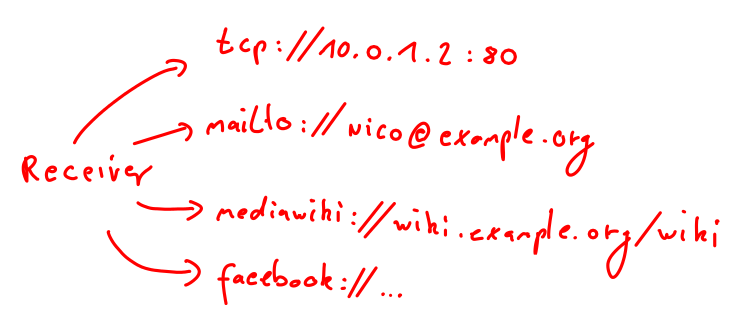
\includegraphics[scale=0.8]{addressmultiplexing.png}
\end{figure}
Theis multiplexing of addresses allows different transports to be used
for one peer, so that there is a higher diversity in outgoing packets.
% ----------------------------------------------------------------------------
\subsection{Access Methods}
\label{accessmethods}
Transport protocols can either be accessable \textit{directly} or 
\textit{indirectly}. In case of direct access (figure \ref{directaccess})
the sending peer directly connects to the receiving peer.
\begin{figure}
    \centering
    \caption{Direct Access}
    \label{directaccess}
    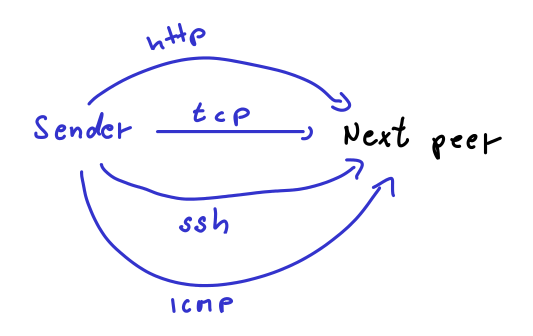
\includegraphics[scale=0.8]{directaccess.png}
\end{figure}
In case of indirect access, the sender stores the postcard on a intermediate
server and the receiving peer polls this server for postcards, as shown
in figure \ref{indirectaccess}.
\begin{figure}
    \centering
    \caption{Indirect Access}
    \label{indirectaccess}
    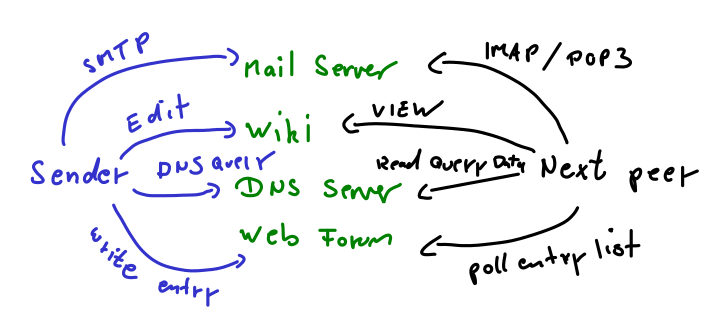
\includegraphics[scale=0.8]{indirectaccess.png}
\end{figure}
% ----------------------------------------------------------------------------
\subsection{List of Supported Transports}
To ensure interoperability, clients which support a specific
protocol version must support all listed transport protocols. This version
supports all protocols specified in table \ref{transportprotocollisting}.
\begin{longtable}{|c|c|c|}
\caption{Transport protocols}
\label{transportprotocollisting}
\\
\hline
\textbf{Protocol} & \textbf{Description} & \textbf{Supported versions}\\
\hline
tcp & Transmission Control Protocol & 0.1 - 0.1\\
\hline
\end{longtable}

\section{Onion Routing}
\label{onionrouting}
Onion routing is used to ensure sender-receiver anonymity. In contrast
to the Tor-network, there are no exit nodes and the receiver can be anyone
in the onion chain (see fig. \ref{onionrouting}).
\begin{figure}
    \centering
    \caption{Onion Routing}
    \label{onionrouting}
    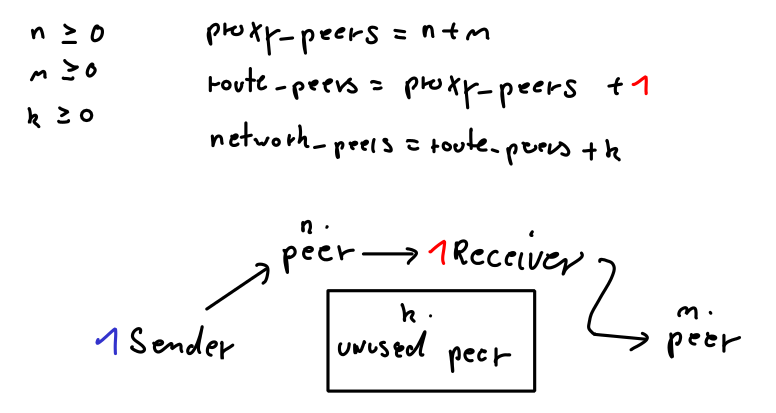
\includegraphics[scale=0.8]{onionrouting.png}
\end{figure}
The peers between the sender and receiver and after the receiver are
called \textit{proxy peers}. The number of proxy peers between the
sender and the receiver and the number of proxy peers after receiver
can range from from 0 up to the maximum number of proxy peers. The sum
of both proxy peers is the \textit{chosen number of proxy peers} and
usually stays consistent for one peer.

The recommended number of proxy peers is \textbf{5}, as a tradeoff between
latency, bandwidth and anonymity. Section \ref{noise}, p. \pageref{noise}
explains in detail why 5 is the recommended number.
% BT: ok
% ----------------------------------------------------------------------------
\subsection{Source Based Routing}
Before creation of an onion, a random route to the receiver is generated.
The route is calculated as follows:
\begin{enumerate}
\item Select random peers from known peer times the number of required proxy peers
\item Shuffle and insert the receiver at a random position
\item Retrieve a random transport protocol address from each peer
\end{enumerate}
For each onion, a new random routes must be calculated.
% ----------------------------------------------------------------------------
\subsection{Onions}
\label{eofonion}
Onions are building the base for the EOF protocol.
The EOF messages described in section \ref{eofmessages}
are multiple times encrypted and assembled according to 
the previously calculated random route. 
The result is called an \textit{onion} and
an example onion is shown in figure \ref{onion}.
\begin{figure}
    \centering
    \caption{An Onion (2 and 3 layers)}
    \label{onion}
    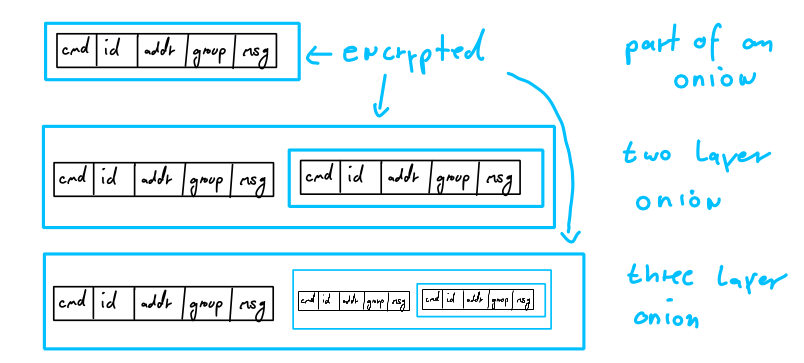
\includegraphics[scale=0.8]{onion.png}
\end{figure}
%% An onion packet is a (multiple times) encrypted packet.
%% An onion packet contains at least one plaintext packet, but can also contain
%% already encrypted packets. It may look like as follows:
Every layer of an onion is encrypted for the specific peer
and the previous encrypted layer is appended after the EOF message
in reencrypted.
In case the onion layer contains the EOF message
3002 or 3003, the layer should also be signed. In all other
cases the onion layer should only be encrypted.
\begin{enumerate}
\item Create EOF message for the last peer
\item Encrypt EOF message for the last peer (first and innermost onion layer)
\item Redo steps one and two for every peer, but append the previous result
\end{enumerate}
% ----------------------------------------------------------------------------
\subsection{Packet Sizes}
The average packet size depending on the number of peers it was
(re-)encrypted for can be found in table \ref{pkgsizes}.
It was generated by running the reference implementation\\
(\verb=ceof onion -m "test" peer0  | wc -c=)
and increasing the number of proxy peers to be inserted.
The resulting size includes the final onion, 
but does not include transport protocol headers.
\begin{longtable}{|c|c|}
\caption{Packet sizes (experimental)}
\label{pkgsizes}\\
\hline
\textbf{Proxy peers} & \textbf{Packet size (in KiBiBytes)}\\
\hline
\textbf{1} & 1.2\\
\hline
\textbf{2} & 1.9\\
\hline
\textbf{3} & 2.6\\
\hline
\textbf{4} & 3.3\\
\hline
\textbf{5} & 4.0\\
\hline
\textbf{6} & 4.8\\
\hline
\textbf{7} & 5.6\\
\hline
\textbf{8} & 6.3\\
\hline
\textbf{9} & 7.1\\
\hline
\textbf{10} & 8.0\\
\hline
\end{longtable}

\section{Noise}
\label{noise}
Noise is being used to constantly send out data on the network.
This prevents statistical analysis of the behaviour of a user and makes
de-anonymisation more impractical due to the amount of data that needs
to be tracked and analysed.
%There are many situations in which an EOFi sends out data to the network,
%although you did not write a message: In fact, as EOFi \textbf{always}
%sends packets in a fixed interval, it needs to have data to encrypt and send.
Furthermore, noise is used to fill in the unused fields in the EOF messages.
Noise can be any type of random data. As the current random number generators
are quite expensive, it is recommend to use a dictionary like old 
messages, log files, public emails, etc. for noise input.
The reference implementation uses the archive of RFCs as base for noise.
The noise workflow is shown in figure \ref{noiseworkflow}.
\begin{figure}
    \centering
    \caption{Noise Workflow}
    \label{noiseworkflow}
    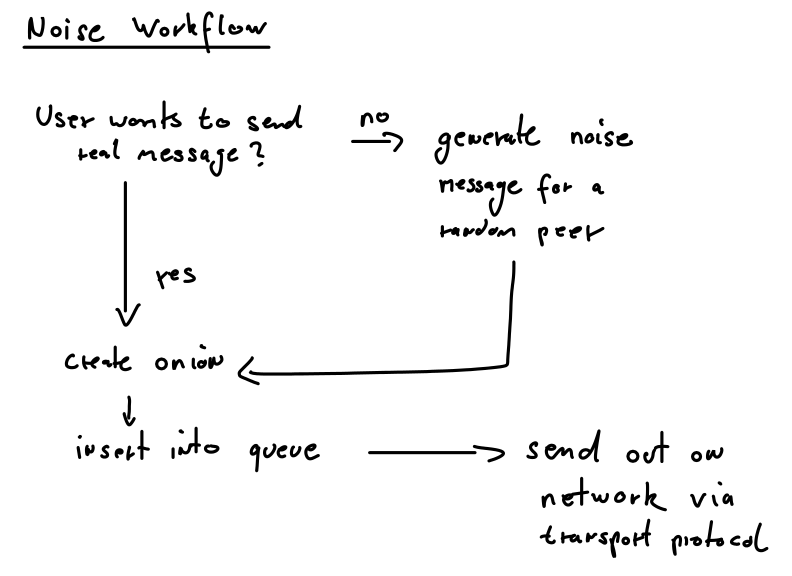
\includegraphics[scale=0.8]{noiseworkflow.png}
\end{figure}
% ----------------------------------------------------------------------------
\subsection{Latency}
\label{latency}
It is important for the user experience of the chat system to minimise latency.
This is especially important after the initial \textit{human handshake}
of saying hello has been made (before that nobody knows when to expect
a message).
The paper about
\textit{System Response Time and User Satisfaction}\cite{responsetime}
indicates that response times up to 6 seconds are tolerable. These numbers
cannot be related directly to the tolerated delay, because the receiving
peer does not exactly know when the sending peer wrote a message.
Every additional proxy peers adds an amount of time to the latency until the
message arrives, as can be seen below.
% ----------------------------------------------------------------------------
\subsubsection{Average Latency}
The average latency for a peer is calculated as follows:
$$\frac{\sum\limits_{i=0}^{(Proxy peers count +1)}}{Proxy peers count + 1}$$
An additional count (+1) is needed to include the receiving peer itself.
Depending on the sending interval this results in different average
waiting times for a message to arrive, as expressed in
the following formula:
$$Intervaltime * \frac{\sum\limits_{i=0}^{(Proxy peers +1)}}{Proxy peers + 1}$$
The average latency depending on the number of hosts and the sending interval
used is shown in table \ref{avglatencypeers}.
\begin{longtable}{|c|c|c|c|c|c|c|}
\caption{Average latency based on number of proxy peers}
\label{avglatencypeers}\\
\hline
\multirow{2}{*}{\textbf{Proxy peers}} & \multicolumn{6}{|l|}{\textbf{Average latency (multiplied by delay times)}} \\
& \textbf{(\# timeslots)} & \textbf{0.125s} & \textbf{0.25s} & \textbf{0.5s} & \textbf{1s} & \textbf{2s}\\
\hline
\textbf{1} & 0.5 & 0.0625s & 0.125s & 0.25s & 0.5s & 1s\\
\hline
\textbf{2} & 1 & 0.125s & 0.25s & 0.5s & 1s & 2s\\
\hline
\textbf{3} & 1.5 & 0.1875s & 0.375s & 0.75s & 1.5s & 3s\\
\hline
\textbf{4} & 2 & 0.25s & 0.5s & 1s & 2s & 4s\\
\hline
\textbf{5} & 2.5 & 0.3125s & 0.625s & 1.25s & 2.5s & 5s\\
\hline
\textbf{6} & 3 & 0.375s & 0.75s & 1.5s & 3s & 6s\\
\hline
\textbf{7} & 3.5 & 0.4375s & 0.875s & 1.75s & 3.5s & 7s\\
\hline
\textbf{8} & 4 & 0.5s & 1s & 2s & 4s & 8s\\
\hline
\textbf{9} & 4.5 & 0.5625s & 1.125s & 2.25s & 4.5s & 9s\\
\hline
\textbf{10} & 5 & 0.625s & 1.25s & 2.5s & 5s & 10s\\
\hline
\end{longtable}
% ----------------------------------------------------------------------------
\subsubsection{Maximum Latency}
Furthermore besides the average latency, the maximum latency needs
to be taken into account as well, which is shown in table \ref{maxlatencypeers}.
\begin{longtable}{|c|c|c|c|c|c|c|}
\caption{Maximum latency based on number of proxy peers}
\label{maxlatencypeers}\\
\hline
\multirow{2}{*}{\textbf{Proxy peers}} & \multicolumn{6}{|l|}{\textbf{Maximum latency (multiplied by delay times)}} \\
& \textbf{(\# timeslots)} & \textbf{0.125s} & \textbf{0.25s} & \textbf{0.5s} & \textbf{1s} & \textbf{2s}\\
\hline
\textbf{1} & 1 & 0.125s & 0.25s & 0.5s & 1s & 2s\\
\hline
\textbf{2} & 2 & 0.25s & 0.5s & 1s & 2s & 4s\\
\hline
\textbf{3} & 3 & 0.375s & 0.75s & 1.5s & 3s & 6s\\
\hline
\textbf{4} & 4 & 0.5s & 1s & 2s & 4s & 8s\\
\hline
\textbf{5} & 5 & 0.625s & 1.25s & 2.5s & 5s & 10s\\
\hline
\textbf{6} & 6 & 0.75s & 1.5s & 3s & 6s & 12s\\
\hline
\textbf{7} & 7 & 0.875s & 1.75s & 3.5s & 7s & 14s\\
\hline
\textbf{8} & 8 & 1s & 2s & 4s & 8s & 16s\\
\hline
\textbf{9} & 9 & 1.125s & 2.25s & 4.5s & 9s & 18s\\
\hline
\textbf{10} & 10 & 1.25s & 2.5s & 5s & 10s & 20s\\
\hline
\end{longtable}
% ----------------------------------------------------------------------------
\subsection{Bandwidth Usage}
\label{bwusagetheory}
Based on the calculated packet sizes (section \ref{pkgsizes}, p. \pageref{pkgsizes}), 
the \textbf{minimal outgoing bandwidth capability}, as shown in table \ref{bandwidth},
is required.
The highest needed bandwidth
in case of 10 proxy peers sending at an interval of 0.125s results in 64 KiB/s
(equivalent of 512 KBit/s).
Today DSL connections usually exceed this limit by orders of magnitudes.
\begin{longtable}{|c|c|c|c|c|c|}
\caption{Minimal Outgoing Bandwidth Capability}
\label{bandwidth}\\
\hline
\multirow{2}{*}{\textbf{Proxy peers}} & \multicolumn{5}{|l|}{\textbf{Intervals / Bandwidth usage in KiB/s}} \\
& \textbf{0.125s} & \textbf{0.25s} & \textbf{0.5s} & \textbf{1s} & \textbf{2s}\\
\hline
\textbf{1} & 9.6 & 4.8 & 2.4 & 1.2 & 0.6\\
\hline
\textbf{2} & 15.2 & 7.6 & 3.8 & 1.9 & 0.95\\
\hline
\textbf{3} & 20.8 & 10.4 & 5.2 & 2.6 & 1.3\\
\hline
\textbf{4} & 26.4 & 13.2 & 6.6 & 3.3 & 1.65\\
\hline
\textbf{5} & 32 & 16 & 8 & 4 & 2\\
\hline
\textbf{6} & 38.4 & 19.2 & 9.6 & 4.8 & 2.4\\
\hline
\textbf{7} & 44.8 & 22.4 & 11.2 & 5.6 & 2.8\\
\hline
\textbf{8} & 50.4 & 25.2 & 12.6 & 6.3 & 3.15\\
\hline
\textbf{9} & 56.8 & 28.4 & 14.2 & 7.1 & 3.55\\
\hline
\textbf{10} & 64 & 32 & 16 & 8 & 4\\
\hline
\end{longtable}
Even on mobile networks, HSUPA Category 1 delivers 0.73 Mbit/s upstream bandwidth.
Older ISDN and Modem connections would not suffice,
though today there are a lot of alternative connections available.\cite{wiki:bitrates}
If using only 9 proxy servers with 0.125s delay or
10 proxy servers with a delay of 0.25s, EDGE could be supported.
The total required network bandwidth is the product of peers in the
network multiplied by the outgoing bandwidth per peer:
$$Required Network Bandwidth = Network Peers * Peer Bandwidth$$
Thus in a network with 100 peers, all of them using 10 proxy peers
and sending at a rate of 0.125s, the total required network bandwidth would be
$$RNB = 100 * 64 KiB/s = 6400 KiB/s = 6.25MiB/s = 50 MBit/s$$
If also the receiving side is inside the same network, the required network
bandwidth has to be multiplied by two and thus results in 
\textit{100 MBit/s}. This is exactly half of what a fast Ethernet switch
can deliver, because fast Ethernet provides full duplex 100Mbit/s streams
and thus a single fast Ethernet fabric would support 200 simultaneous users.
As the network bandwidth cannot be controlled or influenced by the user
directly, these calculations may simply indicate the network bandwidth
usage for network providers. The user can focus on the bandwidth requirements
found in table \ref{bandwidth}.
% ----------------------------------------------------------------------------
\subsection{Fixed interval for sending}
To prevent de-anonymisation by doing statistical analysis on the traffic,
postcards are sent at a fixed rate.
In case there is no message to be send, onions with no receiving
peer (\textit{noise}) are used instead.

To avoid problems with different sending intervals
(queuing, buffer exceeding) a network wide fixed sending interval
should be chosen. From the calculations made above, an interval
of \textbf{0.25s} seems to provide a good trade-off between
latency, anonymity and bandwidth usage.

The number of proxy peers can be chosen by every peer individually
and can be used to focus on smaller bandwidth usage and less latency
or a higher degree of anonymity. A value of 5 in a network of 100 peers
would make de-anonymising less probable than winning the game
Lotto (6 out of 49) in Germany (see table \ref{deanontable}).

% ----------------------------------------------------------------------------
\section{Features}
This section describes which features are supported by the chat protocol.
Figure \ref{features-technologies} gives a quick overview of how the
features relate to the used technologies.
\begin{figure}
    \centering
    \caption{Features and Technologies}
    \label{features-technologies}
    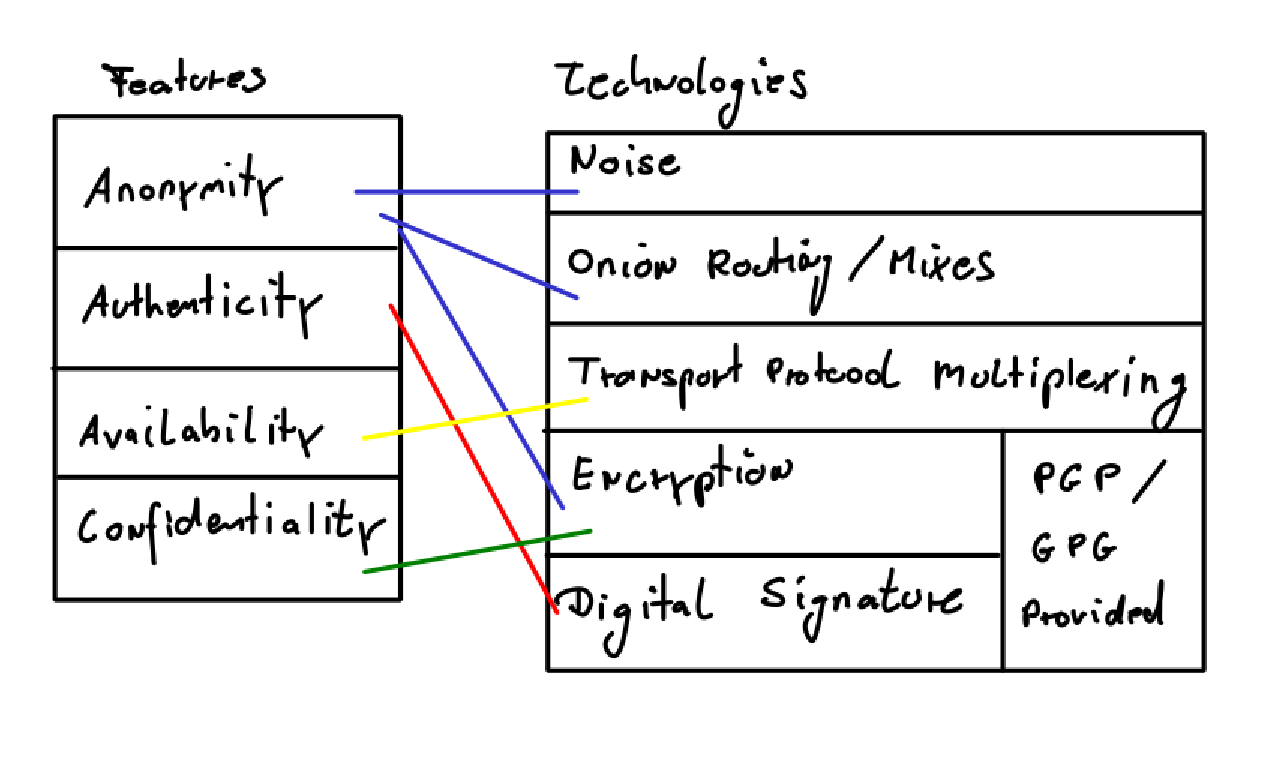
\includegraphics[scale=0.8]{features-technologies.eps}
\end{figure}
% ----------------------------------------------------------------------------
\subsection{Anonymity}
One of the main objectives of this protocol is to provide a chat system that
hides who is talking to whom (\textit{Sender-Receiver Anonymity}). 
In practise there are limits on the degree of anonymity that can be reached.
This protocol specifies the use of
\begin{itemize}
\item Onion Routing (\ref{onionrouting}, p. \pageref{onionrouting}),
\item Noise (\ref{noise}, p. \pageref{noise})
\item and OpenPGP (\ref{openpgp}, p. \pageref{openpgp})
\end{itemize}
to achieve a high degree of anonymity.
% ----------------------------------------------------------------------------
\subsubsection{Degree of Anonymity}
If an attacker controls all hosts that are part of the chat network, 
it is impossible to guarantee anonymity at all.
Thus to allow any degree of anonymity, there must be hosts in the network,
which are not run by the attacker besides the sender and the receiver.
As specified by Onion Routing, there are a number of proxy peers used
to hide the message receiver.

In a network in which the attacker does not run all nodes, there is a probability
that the given route considers only the hosts run by the attacker. As soon as the
route considers at least one different host, the attacker cannot distinguish
between the real recipient and a proxy peer. So we have to consider the probability
that the attacker controls \textbf{all} proxy peers for a given route only.
This probability is the same as the one used to calculate the winning probability
in the game of luck \textit{Lotto}, in which the
winning chances are expressed like this:
$$P_r = \frac{{\binom{6}{r}}{\binom{N-6}{6-r}}}{{\binom{N}{6}}}, r \in \{0, \ldots, 6\}$$
%To remove anonymity, all peers in a route, which are not the 
%sender and the receiver have to be compromised.
Depending on the number of hosts in a network (number of possible
numbers in lotto) and on the number of hosts in a specific route
(number of correct numbers in lotto), the de-anonymisation
probabilities (lotto: winning probabilities) are shown in table \ref{deanontable}.
\begin{longtable}{|c|c|c|c|c|c|}
\caption{De-Anonymisation Probablities (for one packet)}
\label{deanontable}\\
\hline
\textbf{Peers in network /} & \textbf{$10$} & \textbf{$10^2$} & \textbf{$10^3$} & \textbf{$10^4$} & \textbf{$10^5$} \\
\textbf{Proxy peers} & & & & & \\
\hline
\textbf{1} & 1:10 & 1:100 & 1:1000 & 1:10000 & 1:100000\\
\hline
\textbf{2} & 1:45 & 1:4950 & 1:499500 & 1:4.9995e+07 & 1:4.99995e+09\\
\hline
\textbf{3} & 1:120 & 1:161700 & 1:1.66167e+08 & 1:1.66617e+11 & 1:1.66662e+14\\
\hline
\textbf{4} & 1:210 & 1:3.92122e+06 & 1:4.14171e+10 & 1:4.16417e+14 & 1:4.16642e+18\\
\hline
\textbf{5} & 1:252 & 1:7.52875e+07 & 1:8.25029e+12 & 1:8.325e+17 & 1:8.3325e+22\\
\hline
\textbf{6} & 1:210 & 1:1.19205e+09 & 1:1.36817e+15 & 1:1.38681e+21 & 1:1.38868e+27\\
\hline
\textbf{7} & 1:120 & 1:1.60076e+10 & 1:1.94281e+17 & 1:1.97996e+24 & 1:1.98371e+31\\
\hline
\textbf{8} & 1:45 & 1:1.86088e+11 & 1:2.41151e+19 & 1:2.47322e+27 & 1:2.47946e+35\\
\hline
\textbf{9} & 1:10 & 1:1.90223e+12 & 1:2.65802e+21 & 1:2.74583e+30 & 1:2.75474e+39\\
\hline
\textbf{10} & 1:1 & 1:1.73103e+13 & 1:2.6341e+23 & 1:2.74336e+33 & 1:2.75449e+43\\
\hline
\end{longtable}
As can be seen in this table, the probability of an attacker being able to
de-anonymise in a network of 100 peers using 5 proxy peers is less then
the probability of winning Lotto with 6 of 49 (1:13983816).
To support a high chance of not hitting the attackers peers and thus
avoiding de-anonymisation, the number of peers in the network as well 
as the number of proxy peers should be increased as much as possible. 
The number of peers in the network are
depending on how many peers are actually using the network. This can be
increased to a certain degree by adding artificial peers.
The number of proxy peers cannot be increased infinitely, 
as shown in \ref{latency}, p. \pageref{latency}.
% ----------------------------------------------------------------------------
\subsection{Authenticity and Confidentiality}
Digital signatures provide methods to ensure that a given message
was composed by a given public key and that the content has not been
modified. 
The process of encryption protects data from external
viewing and thus ensures the confidentiality of a message.
The features of OpenPGP (\ref{openpgp}, p. \pageref{openpgp})
are being used to guarantee authenticity.
% ----------------------------------------------------------------------------
\subsection{Availability}
To prevent easy denial of service attacks, this protocol specifies various
measurements to make denial of service attacks harder. In particular
the following techniques are used to support the availbility:
\begin{itemize}
\item Transport protocol multiplexing (\ref{multiplexing}, p. \pageref{multiplexing})
\item Transport protocol tunneling (\ref{tunneling}, p. \pageref{tunneling})
\end{itemize}
% ----------------------------------------------------------------------------
\subsection{Direct chat}
This chat protocol supports only direct chat (1:1) as opposed 
to multi user / group chat.

% ----------------------------------------------------------------------------
\section{Implementation}
This section describes the actual implementation
Python?
\subsection{Non-Cross OS Support}
Support for different OS would have made development more
hard, so support for POSIX alike operating systems was targeted.

\subsection{Python-GPG}
Various implementations \cite{python-gpg}
PyMe: 3 Nachrichten in 2010
\url{http://sourceforge.net/mailarchive/forum.php?forum_name=pyme-help&style=threaded}

python-gnupg commits in september 2011 \cite{python-gnupg}

% ----------------------------------------------------------------------------
\section{Test of the Prototype}
    6. Description of test results


\section{Conclusions}
% ------------------------------------------------------------------------------
\subsection{Disadvantages}
Limited traffic like on mobile phones, raise costs and thus me not
fit on them.
% ------------------------------------------------------------------------------
\subsection{Future Work}
Implement Key Exchange.
Cross OS support.

% ----------------------------------------------------------------------------
\appendix
\chapter{UI and User integration}
The following sections have been written and used in a parallel project to
develop a chat UI that is independent on the actual chat server.
The implemented chat ui can be used for chatting with the prototype
implementation.
\label{chatui}
\section{Interface between the chat server and the user interface ("`cs2ui"')}
\label{eofi2ui}
This section specifies the commands used between the user interface (UI)
and chat server (CS).
% Nico: 1.0
% -----------------------------------------------------------------------------
\subsection{Connection}
The chat server provides a TCP listener on port 6667, to which the UI connects 
to. Alternate ports may be used, but need to be specified explicitly.
% -----------------------------------------------------------------------------
\subsection{Commands: Classes and packet description}
All packets exchanged between EOFi and the UI are formatted as
\textit{EOF commands}. EOF commands always begin with 4 bytes, 
which contain a numeric code encoded in UTF-8.

Commands sent by the server begin with \textbf{11}, commands send by the
UI begin with \textbf{21}.
% -----------------------------------------------------------------------------
\subsection{ID}
% -----------------------------------------------------------------------------
\subsection{1100: Acknowledge}
The is a general acknowledge answer. 
The request with the same \emph{ID} as the packet was successful.
\subsubsection{Parameters}
\begin{longtable}{|c|c|c|c|}
\caption{Command 1100 parameters}\\
\hline
\textbf{Parameter} & \textbf{Type} & \textbf{Description} & \textbf{Example}\\
\hline
ID & EOFsdt: id & packet id & afdb12\\
\hline
\end{longtable}
\subsubsection{Example}
\begin{verbatim}
1100abfudh
\end{verbatim}
% Nico: 1.0
% -----------------------------------------------------------------------------
\subsection{1101: Failure}
The is a general failure answer. The request with the
same \emph{ID} as the packet failed.
Details are specified in the reason message.
\subsubsection{Parameters}
\begin{longtable}{|c|c|c|c|}
\caption{Command 1101 parameters}\\
\hline
\textbf{Parameter} & \textbf{Type} & \textbf{Description} & \textbf{Example}\\
\hline
ID & EOFsdt: id & packet id & afdb12\\
\hline
Reason & EOFsdt: msgtxt & Why the connection was refused & Too many UIs connected.\\
\hline
\end{longtable}
If the failed command was "`2100"', EOFi will close the socket afterwards.
\subsubsection{Example}
\begin{verbatim}
1101abfudhSome error\0\0\0\0\0\0\0\0\0\0\0\0\0\0\0\0\0\0\0\0\0\0\0\0\0\0\0
\0\0\0\0\0\0\0\0\0\0\0\0\0\0\0\0\0\0\0\0\0\0\0\0\0\0\0\0\0\0\0\0\0\0\0\0\0
\0\0\0\0\0\0\0\0\0\0\0\0\0\0\0\0\0\0\0\0\0\0\0\0\0\0\0\0\0\0\0\0\0\0\0\0\0
\0\0\0\0\0\0\0\0\0
\end{verbatim}
% Nico: 1.0
% -----------------------------------------------------------------------------
\subsection{1102: Exit requested}
This is a  shutdown request to the UI.
After this message EOFi will exit and there is no communication possible.
\subsubsection{Parameters}
\begin{longtable}{|c|c|c|c|}
\caption{Command 1102 parameters}\\
\hline
\textbf{Parameter} & \textbf{Type} & \textbf{Description} & \textbf{Example}\\
\hline
ID & EOFsdt: id & packet id & afdb12\\
\hline
\end{longtable}
\subsubsection{Example}
\begin{verbatim}
1102abf93a
\end{verbatim}
% Nico: 1.0
% -----------------------------------------------------------------------------
\subsection{1103: Recieved message}
This message is issued by EOFi, if a message is received.
\subsubsection{Parameters}
\index{Command!1103}
\begin{longtable}{|c|c|c|c|}
\caption{Command 1103 parameters}\\
\hline
\textbf{Parameter} & \textbf{Type} & \textbf{Description} & \textbf{Example}\\
\hline
ID & EOFsdt: id & packet id & afdb12\\
\hline
nick & EOFsdt & The sender & telmich\\
\hline
msgtext & EOFsdt & The message & Hallo, mein Freund!\\
\hline
\end{longtable}
\subsubsection{Example}
\begin{verbatim}
1103abfudhtelmich\0\0\0\0\0\0\0\0\0\0\0\0\0\0\0\0\0\0\0\0\0\0\0\0\0\0\0\0\0
\0\0\0\0\0\0\0\0\0\0\0\0\0\0\0\0\0\0\0\0\0\0\0\0\0\0\0\0\0\0\0\0\0\0\0\0\0
\0\0\0\0\0\0\0\0\0\0\0\0\0\0\0\0\0\0\0\0\0\0\0\0\0\0\0\0\0\0\0\0\0\0\0\0\0
\0\0\0\0\0\0\0\0\0\0Hallo!\0\0\0\0\0\0\0\0\0\0\0\0\0\0\0\0\0\0\0\0\0\0\0\0
\0\0\0\0\0\0\0\0\0\0\0\0\0\0\0\0\0\0\0\0\0\0\0\0\0\0\0\0\0\0\0\0\0\0\0\0\0
\0\0\0\0\0\0\0\0\0\0\0\0\0\0\0\0\0\0\0\0\0\0\0\0\0\0\0\0\0\0\0\0\0\0\0\0\0
\0\0\0\0\0\0\0\0\0\0\0\0\0\0\0\0
\end{verbatim}
\subsubsection{Possible answers}
\begin{itemize}
\item None: EOFi does not resend this packet if the UI lost it.
\end{itemize}
% Nico: 1.0
% -----------------------------------------------------------------------------
\subsection{1104: List of peers}
This is the answer to command \emph{2106} and thus contains the
same ID, as the \emph{2106} request command.
\subsubsection{Parameters}
\begin{longtable}{|c|c|c|c|}
\caption{Command 1104 parameters}\\
\hline
\textbf{Parameter} & \textbf{Type} & \textbf{Description} & \textbf{Example}\\
\hline
ID & EOFsdt: id & packet id & afdb12\\
\hline
Number of peers (nop) & EOFsdt: size & How many peers follow & 20\\
\hline
$nop * Peer$ & EOFsdt: nick & The nickname & telmich\\
\hline
\end{longtable}
The last field is repeated as many times as specified in number of peers.
% Nico: 1.0
% -----------------------------------------------------------------------------
\subsection{1105: Peer information}
This is the answer to command \emph{2105} and thus contains the
same ID, as the \emph{2105} request command.
\subsubsection{Parameters}
\begin{longtable}{|c|c|c|c|}
\caption{Command 1105 parameters}\\
\hline
\textbf{Parameter} & \textbf{Type} & \textbf{Description} & \textbf{Example}\\
\hline
ID & EOFsdt: id & packet id & afdb12\\
\hline
Keyid & EOFsdt:keyid & This peers pgp-keyid & 389E5481065EAA253...\\
\hline
Number of addresses (noa) & EOFsdt: size & & 1\\
\hline
$noa * address$ & EOFsdt: addr & Adress of peer & tcp:127.0.0.1:4243\\
\hline
\end{longtable}
The last field is repeated as often, as specified in the number of addresses
field.
% Nico: 1.0
% -----------------------------------------------------------------------------
\subsection{1106: Peer renamed}
This is the answer to command \emph{2104} and thus contains the
same ID, as the \emph{2104} request command. It is sent out to
\textbf{all} connected user interfaces.
\subsubsection{Parameters}
\begin{longtable}{|c|c|c|c|}
\caption{Command 1106 parameters}\\
\hline
\textbf{Parameter} & \textbf{Type} & \textbf{Description} & \textbf{Example}\\
\hline
ID & EOFsdt: id & packet id & afdb12\\
\hline
Oldnick & EOFsdt & Old nick name & susi\\
\hline
Newnick & EOFsdt & New nick name & heinz\\
\hline
\end{longtable}
\subsubsection{Possible answers}
\begin{itemize}
\item None
\end{itemize}
% Nico: 1.0
% -----------------------------------------------------------------------------
\subsection{2100: Register user interface}
This must be the \emph{first} message sent by the UI. If the answer is not
\emph{1100}, the UI should close the socket afterwards.

\subsubsection{Parameters}
\begin{longtable}{|c|c|c|c|}
\caption{Command 2100 parameters}\\
\hline
\textbf{Parameter} & \textbf{Type} & \textbf{Description} & \textbf{Example}\\
\hline
ID & EOFsdt: id & packet id & afdb12\\
\hline
Name & EOFsdt: UINAME & Name of the UI & ceofui\\
\hline
\end{longtable}

\subsubsection{Possible answers}
\begin{itemize}
\item 1100
\item 1101
\end{itemize}
% Nico: 1.0
% -----------------------------------------------------------------------------
\subsection{2101: Deregister user interface}

\subsubsection{Parameters}
\begin{itemize}
\item none
\end{itemize}

\subsubsection{Possible answers}
\begin{itemize}
\item none
\end{itemize}

EOFi will close the connection to the UI after receiving this message.

% Nico: 1.0
% -----------------------------------------------------------------------------
\subsection{2102: /peer add}
The UI adds a peer to the list of known peers.

\subsubsection{Parameters}
\index{Command!2102: /peer add}%
\begin{longtable}{|c|c|c|c|}
\caption{2102: /peer add parameters}\\
\hline
\textbf{Parameter} & \textbf{Type} & \textbf{Description} & \textbf{Example}\\
\hline
ID & EOFsdt: id & packet id & afdb12\\
\hline
Nick & EOFsdt: nick & Name you identify the peer with & telmich\\
\hline
Address & EOFsdt: addr & Where we can make the first contact & tcp:10.0.42.42:4242\\
\hline
Keyid & EOFsdt: keyid & PGP fingerprint of the peers key & F27987E34E66...\\
\hline
\end{longtable}

\subsubsection{Possible answers}
\begin{itemize}
\item 1100
\item 1101
\end{itemize}
% Nico: 1.0
% -----------------------------------------------------------------------------
\subsection{2103: /peer send}
The UI wants to submit a message to a peer.

\subsubsection{Parameters}
\index{Command!/peer send}%
\begin{longtable}{|c|c|c|c|}
\caption{2103: /peer send parameters}\\
\hline
\textbf{Parameter} & \textbf{Type} & \textbf{Description} & \textbf{Example}\\
\hline
ID & EOFsdt: id & packet id & afdb12\\
\hline
Nick & EOFsdt: nick & Name you identify the peer with & telmich\\
\hline
Message & EOFsdt: msgtxt & The message itself & Hallo, wie geht es Dir?\\
\hline
\end{longtable}

\subsubsection{Possible answers}
\begin{itemize}
\item 1100
\item 1101
\end{itemize}
% Nico: 1.0
% -----------------------------------------------------------------------------
\subsection{2104: /peer rename}
The UI wants to rename a peer.

\subsubsection{Parameters}
\index{Command!/peer rename}%
\begin{longtable}{|c|c|c|c|}
\caption{/peer rename parameters}\\
\hline
\textbf{Parameter} & \textbf{Type} & \textbf{Description} & \textbf{Example}\\
\hline
ID & EOFsdt: id & packet id & afdb12\\
\hline
Oldnick & EOFsdt & Old nick name & susi\\
\hline
Newnick & EOFsdt & New nick name & heinz\\
\hline
\end{longtable}

\subsubsection{Possible answers}
\begin{itemize}
\item 1106
\item 1101
\end{itemize}

% -----------------------------------------------------------------------------
\subsection{2105: /peer show}
The UI requests details about a peer.

\subsubsection{Parameters}
\begin{longtable}{|c|c|c|c|}
\caption{2105: /peer show parameters}\\
\hline
\textbf{Parameter} & \textbf{Type} & \textbf{Description} & \textbf{Example}\\
\hline
ID & EOFsdt: id & packet id & afdb12\\
\hline
Nick name & EOFsdt & Nick name, as known by EOFi & karl-otto\\
\hline
\end{longtable}

\subsubsection{Possible answers}
\begin{itemize}
\item 1101
\item 1105
\end{itemize}
% Nico: 1.0
% -----------------------------------------------------------------------------
\subsection{2106: /peer list}
The UI requests the list of known peers.

\subsubsection{Parameters}
\begin{longtable}{|c|c|c|c|}
\caption{2106: /peer list parameters}\\
\hline
\textbf{Parameter} & \textbf{Type} & \textbf{Description} & \textbf{Example}\\
\hline
ID & EOFsdt: id & packet id & afdb12\\
\hline
\end{longtable}

\subsubsection{Possible answers}
\begin{itemize}
\item 1101
\item 1104
\end{itemize}
% Nico: 1.0
% -----------------------------------------------------------------------------
\subsection{2199: /quit}
The user interface requests EOFi and all other EOFs to exit.
The EOFi will not answer, but send an exit request to all other
EOFs.

\subsubsection{Parameters}
\begin{longtable}{|c|c|c|c|}
\caption{2199: /quit parameters}\\
\hline
\textbf{Parameter} & \textbf{Type} & \textbf{Description} & \textbf{Example}\\
\hline
ID & EOFsdt: id & packet id & afdb12\\
\hline
\end{longtable}

\subsubsection{Possible answers}
\begin{itemize}
\item none
\end{itemize}
% Nico: 1.0


\section{The User Interface ("`ui2user"')}
This section specifies the appereance of the user interface to the user.

% Nico: 1.0
%---------------------------------------------------------------------
\subsection{Interface}
The UI is running as a ncurses application and prompts for input
on a specific line.\footnote{Example output can be found in figure \ref{startup}.}
All commands start with "/".
\begin{figure}[htbp]
    \caption{UI Startup Screen}
    \label{startup}
    \centering
    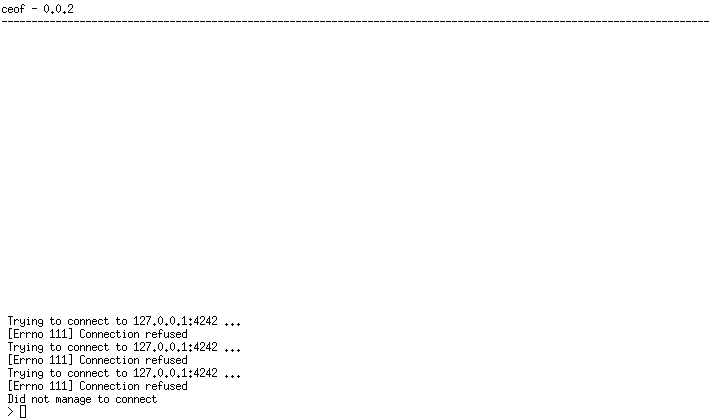
\includegraphics[width=10cm]{ui-startup.png}
\end{figure}

%---------------------------------------------------------------------
\subsection{UI Command: /help}
The /help command prints a short usage
description.\footnote{Example output can be found in figure \ref{help}.}

\subsubsection{Example}
\begin{verbatim}
/help
\end{verbatim}
\begin{figure}[htbp]
    \caption{UI Help Output}
    \label{help}
    \centering
    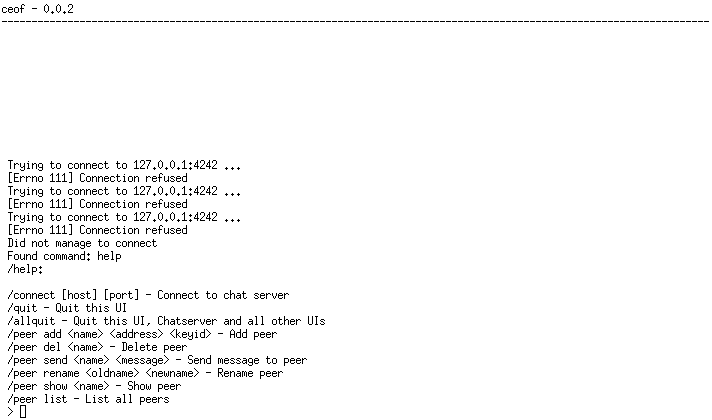
\includegraphics[width=10cm]{help-command.png}
\end{figure}

%---------------------------------------------------------------------
\subsection{UI Command: /connect $[$host$]$ $[$port$]$}
The connect command can be used to connect to the chat
server.\footnote{Example output can be found in figure \ref{connect}.}
Host and port are optional. If omitted, the saved host and/or
port will be used. This command uses message 2100.
\begin{figure}[htbp]
    \caption{UI /connect}
    \label{connect}
    \centering
    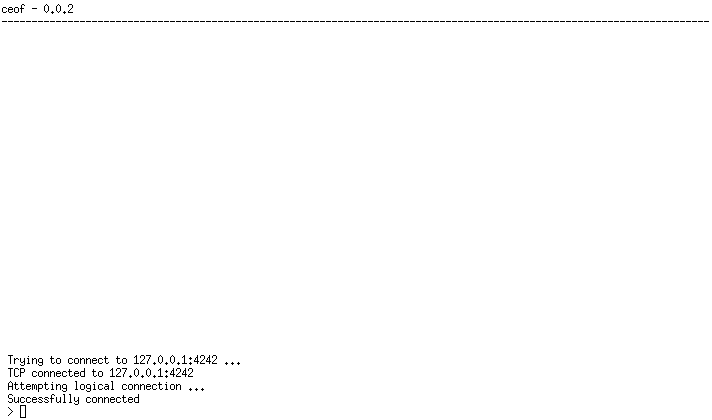
\includegraphics[width=10cm]{connected-to-cs.png}
\end{figure}

\subsubsection{Example}
\begin{verbatim}
/connect 127.0.0.1 4242
\end{verbatim}
% Nico: Code & Doc
%---------------------------------------------------------------------
\subsection{UI Command: /quit}
Request the user interface to exit. It will deregister from the CS.
This command uses message 2101.
\subsubsection{Example}
\begin{verbatim}
/quit
\end{verbatim}
% Nico: 1.0
%---------------------------------------------------------------------
\subsection{UI Command: /allquit}
The UI tells the CS and all connected UIs (including itself) to quit.
This command uses message 2199.\footnote{Example output can be found in figure \ref{allquit}.}
\begin{figure}[htbp]
    \caption{UI /allquit}
    \label{allquit}
    \centering
    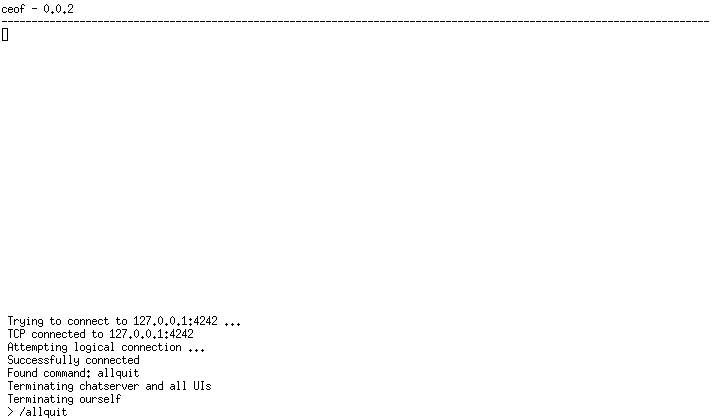
\includegraphics[width=10cm]{allquit.png}
\end{figure}

\subsubsection{Example}
\begin{verbatim}
/allquit
\end{verbatim}
% Nico: 1.0
%---------------------------------------------------------------------
\subsection{UI Command: /peer add $<$name$>$ $<$address$>$ $<$keyid$>$}
Add the peer with the given name \textit{name} to the list
of known peers.\footnote{Example output can be found in figure \ref{peeradd}.}
\begin{figure}[htbp]
    \caption{UI /peer add}
    \label{peeradd}
    \centering
    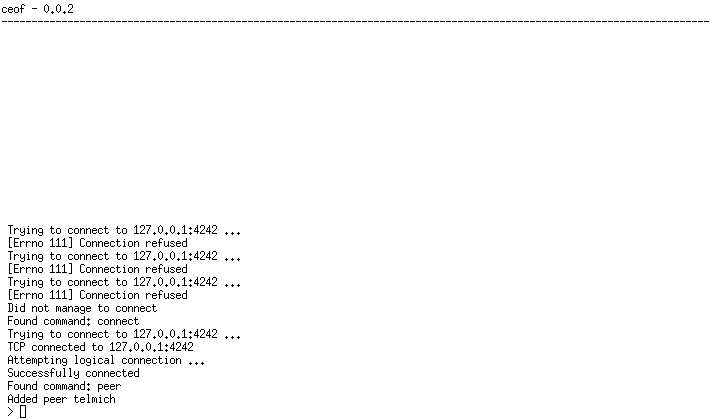
\includegraphics[width=10cm]{peer-add.png}
\end{figure}


\index{UI Command!/peer add}%
\begin{longtable}{|c|c|c|c|}
\caption{UI Command: /peer add parameters}\\
\hline
\textbf{Parameter} & \textbf{Type} & \textbf{Description} & \textbf{Example}\\
\hline
Peer name & EOFsdt: name & Name you identify the peer with & telmich\\
\hline
Address & EOFsdt: address & Where we can make the first contact & tcp://10.0.42.42:4242\\
\hline
Keyid & EOFsdt: keyid & The PGP fingerprint of the peers public key & F27987E34E66...\\
\hline
\end{longtable}

\subsubsection{Example}
\begin{verbatim}
/peer add telmich tcp//:10.0.42.42:4242 F27987E34E7866B2BA39C2FD793EB8FC325251FE
\end{verbatim}
% Nico: 1.0
%---------------------------------------------------------------------
%\clearpage
\subsection{UI Command: /peer del $<$name$>$}
Delete the peer with the given name \textit{name} from the list of
known peers.\footnote{Example output can be found in figure \ref{peerdel}.}
\begin{figure}[htbp]
    \caption{UI /peer del}
    \label{peerdel}
    \centering
    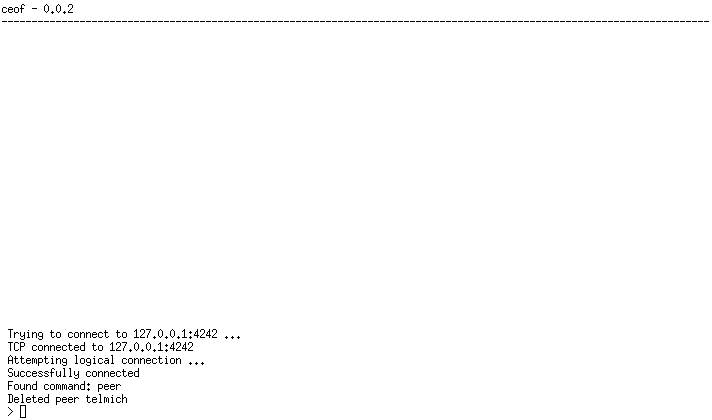
\includegraphics[width=10cm]{peer-del.png}
\end{figure}


\index{UI Command!/peer del}%
\begin{longtable}{|c|c|c|c|}
\caption{UI Command: /peer del parameters}\\
\hline
\textbf{Parameter} & \textbf{Type} & \textbf{Description} & \textbf{Example}\\
\hline
Peer name & EOFsdt: name & Name you identify the peer with & telmich\\
\hline
\end{longtable}

\subsubsection{Example}
\begin{verbatim}
/peer del telmich
\end{verbatim}
% Nico: 1.0
%---------------------------------------------------------------------
%\clearpage
\subsection{UI Command: /peer send $<$name$>$ $<$msgtext$>$}
Send message \textit{msgtext} to peer
\textit{name}.\footnote{Example output can be found in figure \ref{peersend}.}
\begin{figure}[htbp]
    \caption{UI /peer send}
    \label{peersend}
    \centering
    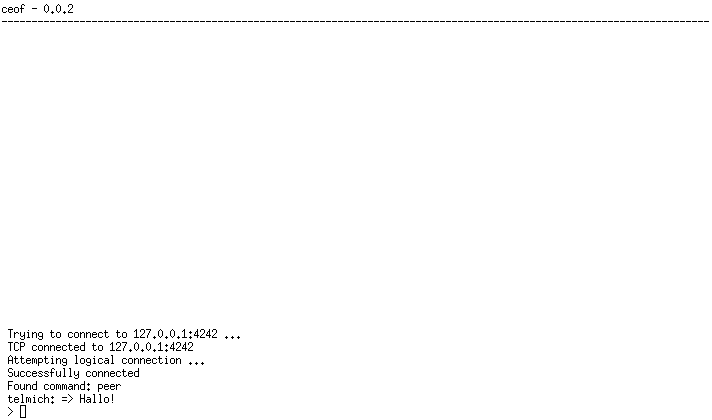
\includegraphics[width=10cm]{peer-send.png}
\end{figure}
\clearpage
\index{UI Command!/peer send}%
\begin{longtable}{|c|c|c|c|}
\caption{UI Command: /peer send parameters}\\
\hline
\textbf{Parameter} & \textbf{Type} & \textbf{Description} & \textbf{Example}\\
\hline
Name & EOFsdt: name & Name you identify the peer with & telmich\\
\hline
Msgtext & EOFsdt: msgtxt & The message itself & Hallo, wie geht es Dir?\\
\hline
\end{longtable}
\subsubsection{Example}
\begin{verbatim}
/peer send telmich Hallo, wie geht es Dir?
\end{verbatim}
% Nico: 1.0
%---------------------------------------------------------------------
%\clearpage
\subsection{UI Command: /peer rename $<$oldname$>$ $<$newname$>$}
Renames the peer.\footnote{Example output can be found in figure \ref{peerrename}.}
\begin{figure}[htbp]
    \caption{UI /peer rename}
    \label{peerrename}
    \centering
    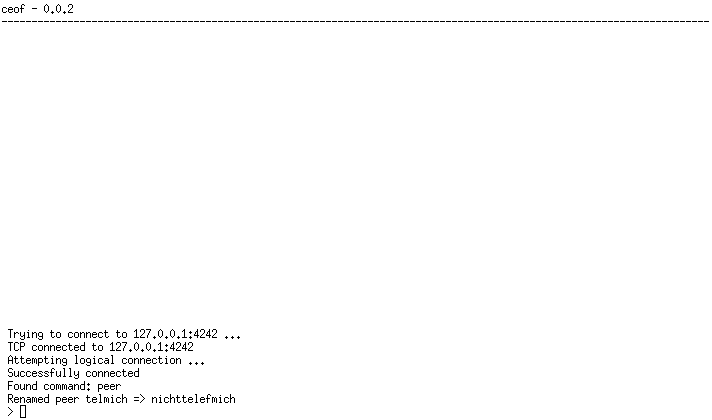
\includegraphics[width=10cm]{peer-rename.png}
\end{figure}


\index{UI Command!/peer rename}%
\begin{longtable}{|c|c|c|c|}
\caption{UI Command: /peer rename parameters}\\
\hline
\textbf{Parameter} & \textbf{Type} & \textbf{Description} & \textbf{Example}\\
\hline
Oldname & EOFsdt: name & Old name & susi\\
\hline
Newname & EOFsdt: name & New name & heinz\\
\hline
\end{longtable}

\subsubsection{Example}
\begin{verbatim}
/peer rename susi heinz
\end{verbatim}
% Nico: 1.0
%---------------------------------------------------------------------
%\clearpage
\subsection{UI Command: /peer show $<$name$>$}
Display detailled information about peer.\footnote{Example output can be found in figure \ref{peershow}.}
\begin{figure}[htbp]
    \caption{UI /peer show}
    \label{peershow}
    \centering
    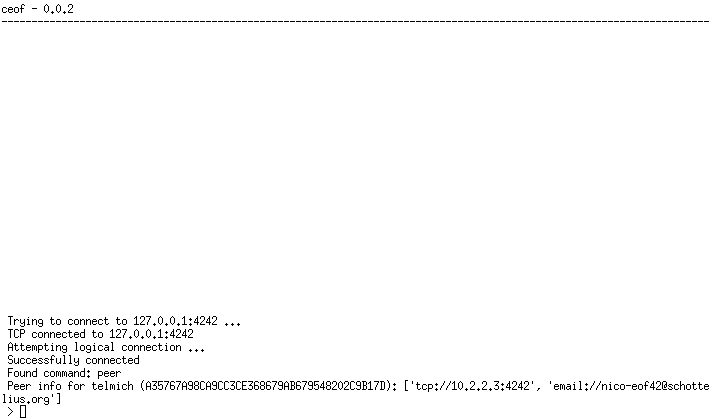
\includegraphics[width=10cm]{peer-show.png}
\end{figure}

\index{UI Command!/peer show}%
\begin{longtable}{|c|c|c|c|}
\caption{UI Command: /peer rename parameters}\\
\hline
\textbf{Parameter} & \textbf{Type} & \textbf{Description} & \textbf{Example}\\
\hline
Peer name & EOFsdt: name & Name as known by CS & karl-otto\\
\hline
\end{longtable}

\subsubsection{Example}
\begin{verbatim}
/peer show karl-otto
\end{verbatim}
% Nico: 1.0
%---------------------------------------------------------------------
%\clearpage
\subsection{UI Command: /peer list}
List of currently known peers. This command does not accept any
parameters.\footnote{Example output can be found in figure \ref{peerlist}.}
\begin{figure}[htbp]
    \caption{UI /peer list}
    \label{peerlist}
    \centering
    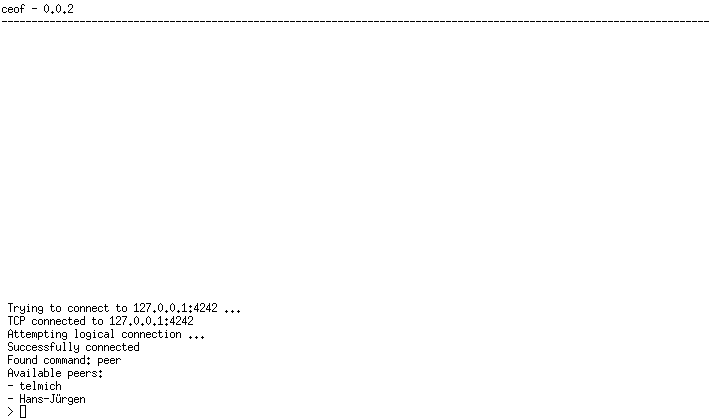
\includegraphics[width=10cm]{peer-list.png}
\end{figure}


\subsubsection{Example}
\begin{verbatim}
/peer list
\end{verbatim}
% Nico: 1.0
% %---------------------------------------------------------------------
% \subsection{Aliases}
% Aliases may optionally be provided by the UI. If an UI provides
% support for aliases, it must implement the "`\emph{/alias}"' command.
% 
% The following aliases should be provided by default,
% to aid new users using EOF.
% % Nico: 1.0
% %---------------------------------------------------------------------
% \subsection{/alias $<aliasname>$ $<command...>$}
% This command should be used to setup aliases.
% % Nico: 1.0
% %---------------------------------------------------------------------
% \subsection{/msg $<name>$ $<msgtext>$}
% Should be an alias for \textit{/peer send $<$name$>$ $<$msgtext$>$}
% % Nico: 1.0
% %---------------------------------------------------------------------
% \subsection{/whois $<name>$}
% Should be an alias for \textit{/peer show $<$name$>$}
% Nico: 1.0

% ----------------------------------------------------------------------------
% \chapter{References}
\begin{thebibliography}{666}
\bibitem{otr} \url{http://www.cypherpunks.ca/otr/}
\bibitem{tor} Tor project, \url{http://www.torproject.org/},
    \url{http://www.icir.org/vern/cs294-28/papers/dingledine.pdf}
\bibitem{tor2} Low-Cost Traffic Analysis of Tor,
    \url{http://www.cl.cam.ac.uk/~sjm217/papers/oakland05torta.pdf}
\bibitem{untrace} Untraceable electronic mail, return addresses, and digital pseudonyms;
    David L. Chaum; 1981;
    \url{http://citeseerx.ist.psu.edu/viewdoc/download?doi=10.1.1.79.7468&rep=rep1&type=pdf}
\bibitem{onion} Onion Routing, \url{http://www.onion-router.net/}
\bibitem{python-gpg} Various implementations for Python,
    \url{http://wiki.python.org/moin/GnuPrivacyGuard}
\bibitem{python-gnupg} python-gnupg - A Python wrapper for GnuPG,
    \url{http://packages.python.org/python-gnupg/}

\bibitem{unused} \url{http://www.privoxy.org/}
\url{https://yro.slashdot.org/story/11/10/08/0326235/russian-telco-mts-bans-skype-other-voip-services}

\url{http://en.wikipedia.org/wiki/Dining_cryptographers_protocol}
\url{http://crypto.stanford.edu/~pgolle/papers/nim.pdf}
\url{http://www.disappearing-inc.com/D/dcnetworks.html}

\bibitem{skype-evil} Urls to decrypt and analyse skype, failing
\url{http://www.disappearing-inc.com/D/dcnetworks.html}

% ---------------------------------------------------------------------- 
\bibitem{icq-wp} ICQ; Wikipedia;
    \url{http://en.wikipedia.org/wiki/ICQ}
% ---------------------------------------------------------------------- 
\bibitem{skype-analysis} An Analysis of the Skype Peer-to-Peer Internet
Telephony Protocol;
Salman A. Baset and Henning G. Schulzrinne;
????

\bibitem{skype-wp} \url{http://en.wikipedia.org/wiki/Skype#Security_and_privacy}
% ---------------------------------------------------------------------- 
% XMPP
% ---------------------------------------------------------------------- 
\bibitem{bandwidth-progress} \url{http://en.wikipedia.org/wiki/Bit_rate#Progress_trends}
\bibitem{bandwidth-list} \url{http://en.wikipedia.org/wiki/List_of_device_bit_rates}

\bibitem{lte} \url{http://en.wikipedia.org/wiki/3GPP_Long_Term_Evolution}

% ---------------------------------------------------------------------- 
% AOL/ICQ/OSCAR
% ---------------------------------------------------------------------- 
\bibitem{oscar} OSCAR \url{http://iserverd.khstu.ru/oscar/}

\bibliographystyle{plain}
\bibliography{nico}
\end{thebibliography}

% ----------------------------------------------------------------------------
\end{document}
